\documentclass[acmsmall]{acmart}

\let\Bbbk\relax % avoid clash: acmart already defines \Bbbk
\usepackage{amssymb,amsfonts}
\usepackage{multirow}
\usepackage{algorithm}
\usepackage{algpseudocode}
\usepackage{tikz}
\usetikzlibrary{arrows.meta,positioning,fit,backgrounds,calc,shapes.geometric}

%% ACM journal metadata --- set to the target venue on submission.
\acmJournal{TOSEM}
\acmYear{2026}
\acmVolume{1}
\acmNumber{1}
\acmArticle{1}
\acmMonth{1}
\acmDOI{}
\copyrightyear{2026}
\setcopyright{rightsretained}
\settopmatter{printacmref=true}

\begin{document}

\title{Does Observability Matter in Cloud-Native Systems? An Empirical Study on Real-Time Anomaly Detection}

\author{Ngoc Duc Anh Nguyen}
\affiliation{%
  \institution{Leeds Beckett University}
  \city{Leeds}
  \country{UK}}
\email{N.Nguyen3896@student.leedsbeckett.ac.uk}

\author{Satish Kumar}
\affiliation{%
  \institution{Leeds Beckett University}
  \city{Leeds}
  \country{UK}}
\email{s.kumar@leedsbeckett.ac.uk}

\author{Nawar Jawad}
\affiliation{%
  \institution{Leeds Beckett University}
  \city{Leeds}
  \country{UK}}
\email{n.jawad@leedsbeckett.ac.uk}

\renewcommand{\shortauthors}{Nguyen et al.}

\begin{abstract}
Cloud-native systems are observable but non-stationary: the telemetry that machine-learning detectors consume is continuously reshaped by deployments, autoscaling and shifting traffic, so a decision boundary that is accurate at training time silently decays in production. Existing studies of observability-driven anomaly detection almost universally evaluate a model that is trained once on a static snapshot, and therefore measure a \emph{stationary ceiling} that may not survive contact with a drifting stream. This paper asks a different question: when the stream drifts, does the \emph{learning paradigm}---static-batch, periodically-retrained, or continuously-online---matter more than the richness of the telemetry, and how do the two interact? We construct a production-representative testbed, TraceFlix, a Kubernetes microservice application instrumented end-to-end with OpenTelemetry, Prometheus, Loki and Tempo, and drive it through four ordered telemetry configurations (metrics-only through full Metrics--Events--Logs--Traces) and four operating regimes that inject realistic drift (latency regression, scale-out, and combined load). On a held-out stationary set, detection quality rises monotonically with telemetry richness (F1 $0.906 \rightarrow 0.994$), with distributed traces the single most valuable signal and ensemble trees the strongest model family; traces also lift root-cause top-1 localisation from $0.91$ to a perfect $1.0$. But under drift the picture inverts: a frozen batch model collapses to F1 $\approx 0.49$--$0.51$ \emph{regardless} of how much telemetry it is given, scheduled retraining recovers only partially (up to $\sim 0.89$), and a lightweight online-adaptive detector dominates at every configuration---and in the large majority of operating regimes---reaching F1 $\approx 0.98$ under full telemetry and even exceeding an all-regimes batch oracle. The online detector is additionally $17$--$32\times$ better on tail latency, $\sim 200$--$550\times$ smaller, and retains no historical data. We conclude that telemetry completeness and continual learning are complementary rather than substitutable: richer signals raise the attainable ceiling, but only adaptation realises it on a live, drifting system.
\end{abstract}

\begin{CCSXML}
<ccs2012>
 <concept>
  <concept_id>10011007.10011074.10011099</concept_id>
  <concept_desc>Software and its engineering~Software reliability</concept_desc>
  <concept_significance>500</concept_significance>
 </concept>
 <concept>
  <concept_id>10010147.10010257.10010258.10010259</concept_id>
  <concept_desc>Computing methodologies~Supervised learning by classification</concept_desc>
  <concept_significance>500</concept_significance>
 </concept>
 <concept>
  <concept_id>10010147.10010178.10010179.10003352</concept_id>
  <concept_desc>Computing methodologies~Online learning settings</concept_desc>
  <concept_significance>500</concept_significance>
 </concept>
 <concept>
  <concept_id>10003456.10010927</concept_id>
  <concept_desc>Social and professional topics~Computing / technology policy</concept_desc>
  <concept_significance>100</concept_significance>
 </concept>
</ccs2012>
\end{CCSXML}
\ccsdesc[500]{Software and its engineering~Software reliability}
\ccsdesc[500]{Computing methodologies~Supervised learning by classification}
\ccsdesc[500]{Computing methodologies~Online learning settings}

\keywords{Observability, anomaly detection, concept drift, online learning, cloud-native systems, machine learning, microservices}

\maketitle

\section{Introduction}\label{sec:intro}
%%===========================================================%%

Cloud-native systems---collections of loosely coupled microservices deployed on container orchestrators such as Kubernetes---have become the dominant architecture for large-scale online services \cite{cncf2024survey}. Their elasticity and rate of change are precisely what make them difficult to operate. A modern deployment may roll out new code many times per day \cite{dora2024}, autoscale pods up and down in response to traffic, reschedule workloads across heterogeneous nodes, and degrade partially in ways that never fully crash any single component. The very properties that make these systems resilient also make their failures diffuse, intermittent and hard to attribute \cite{mohammad2025resilient}. Traditional threshold-based monitoring, in which an operator hand-codes a static alarm for each metric, scales neither to the number of signals nor to the rate at which their normal ranges shift \cite{islam2021,mart2020}.

The response of the field has been \emph{observability}: the practice of instrumenting a system so richly that its internal state can be reconstructed from the telemetry it emits \cite{kosinska2023,boten2022}. The telemetry is conventionally organised into the MELT model---Metrics, Events, Logs and Traces---and a mature observability stack federates all four through vendor-neutral instrumentation such as OpenTelemetry and storage backends such as Prometheus, Loki and Tempo \cite{boten2022,chapman2023}. Observability turns the operational problem into a data problem, and a data problem invites machine learning. A substantial literature now applies classical, deep and graph-based models to observability data, both to \emph{detect} that something has gone wrong and to \emph{localise} the responsible service \cite{lomio2022,dkmak2025,han2024,wang2018,chen2025,raeiszadeh2026}.

Two assumptions run, mostly unexamined, through this literature. The first is that \emph{more telemetry is better}: that adding logs, then traces, then events monotonically improves detection. The second, more consequential, assumption is that the world is \emph{stationary}: that a model trained once on a representative snapshot will continue to perform once it is deployed. Almost every reported result is obtained by training a model on a fixed dataset and evaluating it on a held-out portion of the \emph{same} distribution \cite{lomio2022,dkmak2025,han2024}; the few datasets in common use are themselves narrow, and even on them headline numbers prove fragile under stricter evaluation \cite{landauer2022logsurvey,sarfraz2024quovadis}. This protocol measures what we will call the \emph{stationary ceiling}---the best a detector can do when nothing changes. It is silent on what happens afterwards, when a deployment shifts a service's latency profile, an autoscaler doubles its replica count, or a traffic surge moves every metric's baseline at once. In those moments the data-generating distribution drifts, and a decision boundary fitted to the old normal begins to mislabel the new normal as anomalous.

This paper takes that second assumption as its subject. We argue that for a non-stationary observability stream the dominant design variable is not how much telemetry a detector consumes but \emph{whether and how it keeps learning}. We make this concrete by studying two orthogonal axes together. The first axis is the familiar one of \emph{telemetry completeness}: four ordered configurations from metrics-only to full MELT. The second, which the existing literature rarely treats as a variable at all, is the \emph{learning paradigm}: a static-batch model trained once and frozen; a periodically-retrained model refitted on a sliding buffer; and an online-adaptive model that updates incrementally on every window. Crossing these axes lets us ask not only ``does observability matter?'' but ``\emph{when} does it matter, and compared to what?''

\subsection{Motivating observations}\label{sec:motivation}

A concrete vignette fixes the problem. Suppose a team trains an anomaly detector on a representative week of telemetry and ships it; it performs beautifully in validation. A fortnight later the platform team rolls out a caching change that raises a service's median latency by a modest, entirely healthy margin, and---independently---an autoscaler doubles the service's replicas during a marketing push. Nothing is wrong, but every latency and per-replica-utilisation feature the detector consumes has shifted. The frozen detector, whose notion of ``normal'' was fixed a fortnight ago, now scores this healthy traffic as anomalous and pages the on-call engineer through the night. The team's options are unappealing: silence the detector (losing real coverage), hand-tune thresholds (the very toil observability was meant to remove), or retrain---which lags the next such change by however long the retraining cycle is. This is not a contrived edge case; it is the ordinary weekly life of a cloud-native service, and it is the precise scenario our RQ4 isolates and measures.

Three observations motivate the study. First, instrumentation is not free. Active tracing imposes runtime overhead, and the volume, velocity and variety of telemetry impose real storage and processing costs \cite{kosinska2023,leadingobs,hausenblas2023roi,huang2025mint}. A practitioner choosing how deeply to instrument needs evidence on the \emph{marginal} detection value of each additional pillar, not a blanket assurance that more is better. Second, the field's most recent systematic surveys converge on the same gap from two directions: Raeiszadeh et al.\ \cite{raeiszadeh2026} find that existing detectors ``systematically fail'' on adaptability to dynamic topologies, while Hrusto et al.\ \cite{hrusto2026} find that the great majority of techniques are validated on data that does not represent the drift and heterogeneity of real operations. Adaptability and realistic non-stationarity are exactly the two things a static, single-snapshot evaluation cannot probe. Third, industrial experience reports describe the failure mode directly: at IBM Cloud scale, threshold and static models were found inadequate precisely because ``normal'' is a moving target \cite{islam2021}.

\subsection{Research questions}\label{sec:rqs}

We therefore organise the work around four research questions. The first three characterise the stationary ceiling along the completeness axis---establishing, on our own testbed and under controlled ablation, what the best attainable detection and localisation look like when nothing drifts. The fourth, which is the paper's headline contribution, introduces the temporal axis and asks what survives once the stream moves.

\begin{description}
  \item[\textbf{RQ1 (Completeness ceiling).}] Under stationary conditions, how does the completeness of observability data---metrics-only, ${+}$logs, ${+}$traces, full MELT---affect the accuracy of machine-learning anomaly detection, and which pillar contributes the largest marginal gain?
  \item[\textbf{RQ2 (Model families).}] Which model families best exploit rich, multimodal observability features, and what does that imply for the model that must run in the online setting?
  \item[\textbf{RQ3 (Trace-driven localisation).}] What is the marginal contribution of distributed traces, specifically, to root-cause localisation, holding all other signals constant?
  \item[\textbf{RQ4 (Learning under drift).}] When the telemetry stream is \emph{non-stationary}, how do the static-batch, periodically-retrained and online-adaptive learning paradigms compare on detection quality \emph{and} operational cost, and how does this comparison interact with telemetry completeness?
\end{description}

RQ1--RQ3 are deliberately posed in the established terms of the observability literature, so that our stationary results can be checked against prior expectations; RQ4 then re-uses the \emph{identical} pipeline and feature sets on a drifting stream, so that any reversal of conclusions is attributable to non-stationarity rather than to a change of model, data, or task.

\subsection{Contributions}\label{sec:contributions}

This paper makes the following contributions.

\begin{enumerate}
  \item \textbf{A two-axis experimental design} that crosses telemetry completeness (four nested configurations) with the learning paradigm (static, periodic, online), evaluated on a single production-representative testbed under controlled fault injection and controlled drift. To our knowledge this is the first study to vary \emph{both} the signal set and the learning paradigm while holding the model architecture, feature engineering, fault scenarios and random seed fixed.

  \item \textbf{A characterisation of the stationary ceiling} (RQ1--RQ3) confirming that detection quality rises monotonically with completeness, that distributed traces are the single most valuable increment, that ensemble trees are the strongest model family on multimodal tabular telemetry, and that traces lift root-cause top-1 localisation to perfection on our topology.

  \item \textbf{A drift result that inverts the static conclusion} (RQ4): we show that the frozen batch detector collapses to F1 $\approx 0.49$--$0.51$ on the drifted stream \emph{independently} of how much telemetry it is given, that periodic retraining is a partial and bursty patch, and that a lightweight online-adaptive detector dominates at every configuration and in $10$ of $12$ regime cells, reaching F1 $\approx 0.98$ under full MELT and exceeding an all-regimes batch oracle.

  \item \textbf{An operational-cost analysis} showing the online detector is $17$--$32\times$ better on tail latency, $\sim 200$--$550\times$ smaller in footprint, and retains zero historical data, at the price of modestly higher but smoothly-spent steady-state CPU---reframing the choice of paradigm as a service-level rather than purely accuracy decision.

  \item \textbf{Practical guidance} on minimum-viable observability and on when continual learning is mandatory rather than optional, synthesised into a decision framing for practitioners.
\end{enumerate}

\subsection{Paper organisation}\label{sec:organisation}

Section~\ref{sec:background} reviews observability, anomaly-detection model families, root-cause analysis, concept drift and online learning, and the synthetic-versus-real evaluation divide, closing with the gap we target. Section~\ref{sec:problem} formalises windowed detection and drift and states the two-axis design. Section~\ref{sec:method} describes the TraceFlix testbed, instrumentation, fault injection, the four telemetry configurations, the four drift regimes, the competing learners (including the online model and its adaptation logic), and the evaluation and cost metrics. Section~\ref{sec:results} reports results for RQ1--RQ4. Section~\ref{sec:discussion} discusses why drift is the deciding factor, how completeness and adaptation interact, the operational implications, the relation to prior work, and threats to validity. Section~\ref{sec:conclusion} concludes and outlines future work.

%%===========================================================%%
\section{Background and Related Work}\label{sec:background}
%%===========================================================%%

This section reviews the literature at the intersection of four areas: observability in cloud-native systems (\S\ref{sec:bg-obs}), machine-learning anomaly detection (\S\ref{sec:bg-ad}), observability-driven root-cause analysis (\S\ref{sec:bg-rca}), and---the axis the present work foregrounds---concept drift and online learning over telemetry streams (\S\ref{sec:bg-drift}). Section~\ref{sec:bg-eval} considers the persistent divide between synthetic and operational evaluation, and \S\ref{sec:bg-gap} synthesises the gap.

\subsection{Observability in cloud-native systems}\label{sec:bg-obs}

The term \emph{observability} is borrowed from control theory, where a system is observable if its internal state can be reconstructed in finite time from its outputs \cite{kosinska2023}. Transposed to distributed software, the framing is apt: a microservice mesh is too large, too dynamic and too ephemeral to inspect directly, so its state must be \emph{inferred} from emitted telemetry. Kosi\'nska et al.\ \cite{kosinska2023}, in a systematic mapping of 56 primary studies, establish that cloud-native observability is operationalised through three principal domains---monitoring (metrics), logging, and distributed tracing---and identify a research imbalance in which monitoring receives disproportionate attention relative to logging and tracing. That imbalance matters here because it foreshadows an evaluation imbalance: if most detectors are built and tested on metrics alone, the marginal value of logs and traces is left empirically uncharacterised. More recent surveys confirm and extend this picture for microservice systems specifically, while underlining how quickly the tooling and the threat surface continue to move \cite{faseeha2025observability}.

The practitioner literature crystallises the same three pillars into the MELT model and an end-to-end pipeline: instrumented applications emit telemetry, a vendor-neutral collector (OpenTelemetry) normalises it, backends (Prometheus for metrics, Loki for logs, Tempo for traces) store and index it, and analysis tools query it \cite{boten2022,chapman2023}. The introductory and practice-oriented guides emphasise two themes that bear directly on this paper. First, observability is sold as the foundation for \emph{automated} analysis---alerting, anomaly detection and self-healing---rather than human dashboard-watching \cite{beginnersobs,aws2022obs}. Second, observability is repeatedly described as a \emph{cost} as much as a capability: instrumentation overhead, data-engineering load, and the storage of high-cardinality telemetry are real expenses that a leading practice must manage deliberately \cite{leadingobs,kosinska2023}. The economic premise of our RQ1 follows from this: if each additional pillar carries a cost, practitioners need evidence on its detection benefit.

\subsection{The observability pipeline and its tooling}\label{sec:bg-tooling}

Understanding the cost and the structure of the telemetry on which our detectors operate requires a brief account of the modern observability pipeline, which the practitioner literature documents in depth \cite{boten2022,chapman2023,aws2022obs,beginnersobs}. The contemporary reference design is built around \emph{OpenTelemetry}, an open standard and set of SDKs that has become the de facto vendor-neutral instrumentation layer \cite{boten2022,opentelemetry2024spec}. OpenTelemetry defines a common data model for the three pillars---a metric is a numerical measurement with a timestamp and a set of attributes; a log record is a timestamped, optionally structured event; a span is a timed unit of work within a trace, carrying a trace identifier, a parent identifier, and attributes---and a \emph{collector} that receives, processes and exports this data to backends. The significance of this standardisation for the present study is that the telemetry schema emitted by an OpenTelemetry-instrumented application is the same whether it is generated by a small testbed or a production fleet; building our testbed on OpenTelemetry therefore directly addresses the external-validity concern that synthetic data may not resemble operational data \cite{hrusto2026}.

Boten \cite{boten2022} emphasises that instrumentation is the part of observability with the highest leverage and the highest cost: auto-instrumentation agents capture a baseline of metrics, logs and traces without code changes, but rich, semantically meaningful telemetry---custom metrics, structured log attributes, business-relevant span attributes---requires deliberate engineering. Crucially for our cost argument, tracing is the most expensive pillar to operate. Every request generates a tree of spans; at high request rates this volume is unsustainable to store in full, so production deployments apply \emph{sampling}---head-based (decide at trace start) or tail-based (decide once the trace completes, retaining error traces preferentially). Sampling trades completeness for cost, and the choice of sampling strategy materially affects what trace-derived features a detector can compute; an active research line tries to soften this trade-off with smarter, code- or commonality-aware sampling \cite{huang2025mint,wu2025tracesampling}, or to recover traces without instrumentation at all \cite{ashok2024traceweaver}, and the broader point that observability spend must be justified by return is now made explicitly \cite{hausenblas2023roi}. This is one concrete reason that the marginal detection value of traces (our RQ1, RQ3) is a question with real economic stakes rather than a foregone conclusion.

On the storage and query side, Chapman and Holmes \cite{chapman2023} document the now-common ``LGTM''-style stack---Loki for logs, Grafana for visualisation, Tempo for traces, and a Prometheus-compatible store for metrics---which is exactly the backend topology our testbed adopts (\S\ref{sec:method-testbed}). They stress two operational realities that bear on machine-learning consumers of this data. The first is \emph{cardinality}: metrics are indexed by label sets, and high-cardinality labels (per-user, per-request identifiers) cause a combinatorial explosion in time-series count that dominates storage cost and query latency; feature engineering for detection must therefore aggregate over high-cardinality dimensions rather than consume them raw. The second is the \emph{correlation problem}: metrics, logs and traces are emitted by separate subsystems with separate indices, and joining them---e.g.\ pivoting from an anomalous metric to the trace that explains it---is the central workflow of an investigation and a non-trivial engineering task. A detector that fuses the pillars, as ours does through configuration-aware feature extraction (\S\ref{sec:method-configs}), performs a form of this correlation automatically, which is part of what makes multimodal detection valuable.

The industry guides \cite{aws2022obs,beginnersobs,leadingobs} frame observability less as a tooling choice than as a practice with a maturity curve. A team typically begins with metrics and dashboards (reactive monitoring), adds structured logging, then distributed tracing, and finally invests in correlation, service-level objectives and automated analysis. This maturity progression is, in effect, the completeness axis of our RQ1 made organisational: C1$\rightarrow$C4 traces the same path a team walks as it matures. The guides are also candid that each step up the curve adds cost---more storage, more instrumentation effort, more cognitive load---and that the return on each step is not self-evident \cite{leadingobs}. That candour is precisely the gap our controlled completeness study is designed to fill: to replace the maturity-curve intuition that ``more is better'' with a measured marginal value for each pillar.

\subsection{Anomaly-detection techniques}\label{sec:bg-ad}

Raeiszadeh et al.\ \cite{raeiszadeh2026} provide the most current taxonomy of ML-based anomaly detection for cloud-native architectures and, valuably, evaluate the field against six requirements: adaptability to dynamic topologies, distributed operation, interpretability, scalability with high-velocity telemetry, real-time detection latency, and cross-layer telemetry integration. Their central finding is that existing approaches systematically fail on adaptability, distributed operation and interpretability. We adopt their requirements lens as an evaluative yardstick, and note that \emph{adaptability}---the ability to track a moving distribution---is exactly the requirement a static evaluation cannot test and that RQ4 is designed to probe.

\paragraph{Classical machine learning.} Traditional algorithms---Support Vector Machines, Isolation Forest, Random Forest and gradient-boosted trees---remain competitive for metric-based detection. Lomio et al.\ \cite{lomio2022} train ML models on 168 runtime metrics from Kafka and Zookeeper, reporting AUC above 95\% for performance anomalies with training times of 8--17 minutes. The result is a useful baseline but illustrates the field's characteristic limitations: the evaluation is single-modality and batch, a model trained once on a static snapshot. Neither property survives contact with a streaming, multimodal, non-stationary environment---the point RQ4 makes empirical.

\paragraph{Deep and temporal models.} Deep learning attracts interest for its capacity to model temporal and spatial structure. Dkmak et al.\ \cite{dkmak2025} introduce the \emph{Night's Watch} algorithm, a variational-autoencoder architecture integrating multi-source data with temporal features, reporting precision up to 92\% in microservice anomaly detection. Recurrent architectures (LSTM, GRU) capture temporal dependencies in metric streams, and graph neural networks encode service-topology relations. Across this sub-field an \emph{accuracy--interpretability--cost} trilemma recurs: deep models report strong precision but are opaque (violating the interpretability requirement of \cite{raeiszadeh2026}), are expensive to train, and frequently require the very multimodal data whose marginal value has not been isolated. The literature thus offers increasingly sophisticated \emph{models} while leaving the prior question---how much \emph{signal} they actually need, and whether they can be \emph{kept current}---unanswered.

\paragraph{The recent surge, by modality.} Since then the field has fragmented along the three telemetry pillars, and a brief tour explains why a study that fixes the model and varies the \emph{signal} is overdue. For metrics, deep models for multivariate time series now dominate; recent surveys catalogue an unwieldy zoo of reconstruction-, forecasting-, attention- and contrastive-learning architectures \cite{wang2025mtssurvey,xia2024coupled,choi2024selfsup}, and even the prior question of which metrics actually carry the signal is now studied in its own right \cite{singal2025metric}---even as pointed critiques argue that much of the reported progress is an artefact of flawed evaluation protocols rather than genuine gains \cite{sarfraz2024quovadis,wagner2025metrics}. For logs, the trajectory runs from template-sequence models to pre-trained transformers and, most recently, large language models that read raw log text \cite{landauer2022logsurvey,guan2024logllm,pospieszny2025adalog}. For traces, graph deep learning has become the default, encoding the call graph and its span timings---often fused with metric channels---to surface structural anomalies \cite{chen2023tracegra,akmeemana2025galmad,zhang2025graphneural,alomari2025context}. Each pillar thus has its own thriving sub-literature and its own state of the art, yet the three are seldom measured against one another on the same system---precisely the comparison RQ1 makes.

\paragraph{Multimodal fusion and the LLM turn.} A newer strand fuses the pillars outright. Contrastive and diffusion-based architectures learn a joint representation of metrics, logs and traces and report gains over any single modality \cite{wang2025multimodal,zhang2026modify}, and large multimodal models have begun to serve as few-shot anomaly analysers that ingest heterogeneous signals directly \cite{zhuang2024multimodal}. Beneath all of this sits the broader programme of \emph{AIOps}---machine learning applied to IT operations---whose recent surveys trace the same arc from bespoke models towards general-purpose, LLM-driven pipelines \cite{zhang2024aiops}. Two features of this literature matter here. First, it almost uniformly assumes that more signal is better, without isolating the marginal contribution of each pillar. Second, and more consequentially, it is overwhelmingly \emph{batch}: a model is trained once and scored on a held-out slice of the same distribution, leaving the question of how it behaves once that distribution moves---the subject of RQ4---largely untouched. A few works lean the other way, proposing forecasting- or online-flavoured detectors \cite{xu2024forecasting,wette2024omlad}, and we return to them in \S\ref{sec:bg-drift}.

\paragraph{Observability-integrated, proactive detection.} Mart et al.\ \cite{mart2020} address anomaly detection in Kubernetes clusters using Prometheus metrics, observing that most monitoring remains \emph{reactive}, triggering only once defects are imminent, and proposing time-series forecasting for earlier detection. Their contribution is conceptual as much as technical: it reframes detection as a proactive, observability-integrated capability rather than a threshold alarm---a framing this paper inherits and extends from proactive to \emph{continually self-correcting}.

\subsection{Root-cause analysis through observability data}\label{sec:bg-rca}

Detection is rarely an end in itself; it serves root-cause analysis (RCA), whose effectiveness is tightly coupled to observability quality. Han et al.\ \cite{han2024} propose \emph{HolisticRCA}, formalising RCA along three dimensions---resource-entity localisation (\emph{which} service failed), observability-feature identification (\emph{which} signal indicates it), and fault-type classification (\emph{what kind} of failure)---and using a graph attention network to map heterogeneous trace, metric and log features into a shared space. Their most consequential finding for us is that single-modal RCA is internally inconsistent: a metric-based localiser may implicate one entity while a log-based classifier indicates a different fault type, and jointly modelling all modalities resolves the inconsistency. This is the strongest existing evidence that modalities are \emph{complementary} rather than redundant---but it is demonstrated through a single fused architecture, not a controlled ablation, so the marginal contribution of traces specifically remains entangled with model design. RQ3 isolates it.

Complementary approaches reinforce the value of dependency structure. Wang et al.\ \cite{wang2018} build Bayesian networks from performance metrics (CloudRanger), showing that service-dependency graphs derived from observability data improve fault localisation. Chen et al.\ \cite{chen2025} extend multi-source detection to end-to-end service-function chains (cSFCAD), integrating data-plane and control-plane signals across virtualised network functions. Pedroso et al.\ \cite{pedroso2025} combine LLM-based log analysis with Bayesian networks for probabilistic root-cause inference, demonstrating that language models can extract structure from heterogeneous event data, and---relevant to our fault-injection design---ground their evaluation in controlled fault injection with recorded timestamps. Together these works establish that topology and multi-source fusion improve RCA, yet none varies observability completeness as a controlled factor, and none addresses the temporal validity of the learned model.

The RCA literature has since accelerated sharply---by 2024 a survey already needed to taxonomise dozens of methods \cite{wang2024rcasurvey}. Its centre of gravity has moved towards causal inference and online change-point reasoning, in which a causal graph over services and metrics is constructed and the fault traced back to its source \cite{pham2024rca,yao2024chainofevent,pham2024baro}; a careful benchmark of twenty-one such methods found that the strongest perform well even on short metric windows, but that the ranking is highly method- and dataset-dependent \cite{pham2024rca}. In parallel, large language models have entered RCA both as cloud-incident diagnosers that read mixed telemetry alongside human context \cite{chen2024rca} and as reinforcement-tuned failure localisers \cite{zhang2025thinkfl}. This very activity has exposed how fragile cross-paper comparison remains, prompting dedicated benchmarks built on standardised multimodal telemetry \cite{pham2025rcaeval}. None of it, though, unsettles the two observations above: completeness is not the controlled variable, and the learned model is assumed to remain valid as the system evolves.

\subsection{Concept drift and online learning}\label{sec:bg-drift}

The variable this paper foregrounds is largely absent from the cloud-native anomaly-detection literature but central to the streaming-learning literature, where it has accumulated its own substantial body of surveys \cite{arora2024drift,hovakimyan2024drift,lukats2025drift}. \emph{Concept drift} denotes a change over time in the joint distribution $P(\mathbf{x}, y)$ of features $\mathbf{x}$ and labels $y$. In an observability stream, drift is the norm, not the exception: a deployment changes $P(\mathbf{x} \mid y{=}\text{normal})$ (the same healthy behaviour now produces different metric values), an autoscaling event shifts resource-utilisation baselines, and a traffic surge moves latency and throughput distributions simultaneously. A detector trained on yesterday's normal will, after such a shift, assign high anomaly scores to today's perfectly healthy traffic---a failure mode we term \emph{stale-normal}.

Three families of response exist. A \emph{static} model is trained once and frozen; it is cheap and predictable but, by construction, cannot track drift. A \emph{periodically-retrained} model is refitted at intervals on a sliding window of recent labelled data; it tracks drift in discrete steps but lags by up to one retraining interval, must retain a labelled buffer, and incurs a bursty refit cost. An \emph{online} (incremental) model updates its parameters on every observation via partial fitting; it tracks drift continuously, retains no raw history, and spreads its cost smoothly, at the price of higher aggregate update work and a dependence on a usable label signal. The industrial-scale experience of Islam et al.\ \cite{islam2021} and the adaptability deficit identified by Raeiszadeh et al.\ \cite{raeiszadeh2026} both point to continual learning as the missing ingredient, but neither the surveys nor the primary studies reviewed above evaluate the three paradigms head-to-head on the same observability stream. That head-to-head comparison is RQ4.

The broader stream-learning literature offers a spectrum of online algorithms, and it is worth situating our choice within it. At one end sit incrementally-updated linear models---stochastic-gradient classifiers of the kind our online detector uses---which are cheap, have an $O(d)$ per-update cost, and degrade gracefully, but assume a (locally) linear decision surface. In the middle are incremental decision trees such as the Hoeffding tree and its variants, which grow a tree online using statistical bounds to decide splits; they capture non-linear structure but update less cheaply and are more sensitive to drift in their upper splits. At the adaptive end are explicit drift-detection wrappers (for example windowed change detectors that resize their memory as the stream's error rate shifts) and streaming ensembles that retire and spawn base learners as concepts change. A growing line of work applies exactly these ideas to anomaly detection---incremental autoencoders that re-fit as the stream evolves \cite{li2023autoencoder}, dual drift-detection schemes for anomalous sequences \cite{li2024incremental}, and online learners that are shown to beat their batch counterparts once drift is present \cite{wette2024omlad}; the MLOps community frames the same problem as \emph{model decay} and treats its detection as a first-class monitoring task \cite{leest2025mlmonitoring}. Two design lessons from this literature inform our system. First, \emph{normalisation under drift is as important as the learner}: a model that does not re-centre its inputs will mistake a baseline shift for signal, which is why our detector pairs the classifier with a running normaliser rather than relying on the classifier alone. Second, \emph{adaptation can be implicit or explicit}: our champion bandit is an implicit, lightweight form of the ensemble idea, re-selecting among a small pool by recent performance rather than maintaining a large, costly ensemble. The contribution of RQ4 is not a new online algorithm but a controlled measurement of what \emph{any} reasonable online learner buys, and at what operational cost, relative to the batch paradigms that dominate the cloud-native literature.

\subsection{Monitoring data and real-world evaluation}\label{sec:bg-eval}

Hrusto et al.\ \cite{hrusto2026} provide the field's most recent systematic mapping (104 papers) focused on anomaly detection evaluated with \emph{real-world} monitoring data. Their central argument is methodological: synthetic datasets do not adequately represent the complexity of operational cloud environments, and results obtained on them may not transfer. They taxonomise monitoring data by structure, type and origin, mapping each to suitable preprocessing and detection techniques. Islam et al.\ \cite{islam2021} corroborate this from industrial practice at IBM Cloud scale, finding threshold-based monitoring inadequate for the heterogeneity and scale of real environments---a conclusion their 2025 follow-up reinforces while releasing a public industrial dataset \cite{islam2025cloud}. The community has answered the transferability problem on two fronts. One is a wave of openly released microservice datasets and benchmarks that carry labelled faults across several telemetry modalities \cite{bakhtin2025lo2,pham2025rcaeval,ping2026anomod}, frequently generated through chaos-engineering fault injection whose practice is now mature enough to warrant its own systematic review \cite{owotogbe2026chaos}. The other is a sharper scrutiny of evaluation itself: recent work shows that popular anomaly-detection metrics can reward near-random predictions and that headline gains often evaporate under stricter protocols \cite{sarfraz2024quovadis,wagner2025metrics}, a caution we take seriously in \S\ref{sec:method-metrics}.

This exposes a methodological double bind. Realistic non-stationarity argues for production data, yet \emph{controlled} manipulation of observability completeness \emph{and} drift is only cleanly achievable when the data-generating process is itself controlled---i.e.\ in a testbed with deliberate fault injection and deliberate regime changes. We resolve the bind, as \S\ref{sec:method} details, by using a production-representative testbed (real OpenTelemetry instrumentation and real Prometheus/Loki/Tempo backends) under controlled fault injection \emph{and} controlled drift, rather than either a purely synthetic benchmark or uncontrolled production logs.

\subsection{Synthesis and research gap}\label{sec:bg-gap}

Four convergent gaps emerge.

\begin{description}
  \item[Gap 1 --- Completeness is rarely the controlled variable.] Most techniques are evaluated on a single modality \cite{lomio2022,mart2020}, while the strongest multimodal evidence \cite{han2024} varies the \emph{model} rather than the \emph{signal set}. Few studies hold the model fixed and systematically vary completeness to measure the marginal value of each pillar.
  \item[Gap 2 --- The learning paradigm is almost never a variable.] Evaluation is overwhelmingly single-snapshot batch \cite{lomio2022,dkmak2025,han2024}. The static, periodic and online paradigms are not compared head-to-head on a common observability stream, despite adaptability being a named, unmet requirement \cite{raeiszadeh2026}.
  \item[Gap 3 --- The synthetic-versus-operational divide.] Evaluation is typically either synthetic-and-controlled or operational-and-uncontrolled, rarely both \cite{hrusto2026,islam2021}.
  \item[Gap 4 --- Minimum-viable observability and when to adapt.] There is little practical guidance on either question. Practitioners face a real instrumentation cost \cite{leadingobs,kosinska2023} and a real drift problem \cite{islam2021} with scant evidence to guide either decision.
\end{description}

Table~\ref{tab:positioning} positions the present work against the most directly comparable studies along five axes: whether telemetry completeness is varied as a controlled factor, whether the learning paradigm is varied, whether drift/non-stationarity is evaluated, whether root-cause localisation is addressed, and whether the telemetry is production-representative. No prior study varies both the signal set and the learning paradigm, and none evaluates the three paradigms head-to-head under controlled drift.

\begin{table}[t]
\caption{Positioning against representative prior work. \checkmark\ = addressed; \texttt{part} = partially or implicitly; --- = not addressed.}\label{tab:positioning}
\begin{tabular}{@{}lccccc@{}}
\toprule
Study & Completeness & Paradigm & Drift & RCA & Real telemetry \\
\midrule
Lomio et al.\ \cite{lomio2022}      & ---  & --- & ---  & ---  & \checkmark \\
Mart et al.\ \cite{mart2020}        & ---  & \texttt{part} & --- & --- & \checkmark \\
Dkmak et al.\ \cite{dkmak2025}      & \texttt{part} & --- & --- & \texttt{part} & \checkmark \\
Han et al.\ \cite{han2024}          & \texttt{part} & --- & --- & \checkmark & \checkmark \\
Wang et al.\ \cite{wang2018}        & ---  & --- & --- & \checkmark & \checkmark \\
Chen et al.\ \cite{chen2025}        & \texttt{part} & --- & --- & \checkmark & \checkmark \\
Pedroso et al.\ \cite{pedroso2025}  & \texttt{part} & --- & --- & \checkmark & \checkmark \\
Islam et al.\ \cite{islam2021}      & ---  & \texttt{part} & \texttt{part} & --- & \checkmark \\
\textbf{This work}                  & \checkmark & \checkmark & \checkmark & \checkmark & \checkmark \\
\bottomrule
\end{tabular}
\end{table}

This paper addresses Gap 2 as its primary target (RQ4) and Gaps 1, 3 and 4 as the controlled foundation that makes the RQ4 result interpretable. The design fixes the ML pipeline and varies, orthogonally, the signal set (RQ1--RQ3) and the learning paradigm under drift (RQ4) on a production-representative, fault-injected, drift-controlled testbed.

%%===========================================================%%
\section{Problem Formulation}\label{sec:problem}
%%===========================================================%%

We now make the task and the two design axes precise.

\subsection{Windowed detection}\label{sec:prob-detect}

Let the system emit a continuous multimodal telemetry stream. We discretise time into fixed-length, non-overlapping windows $t = 1, 2, \dots$. For each window a configuration-dependent feature-extraction function $\phi_c$ maps the raw telemetry in that window to a feature vector
\begin{equation}
  \mathbf{x}_t^{(c)} = \phi_c(\text{telemetry}_t) \in \mathbb{R}^{d_c},
\end{equation}
where $c \in \{C1, C2, C3, C4\}$ indexes the telemetry configuration and $d_c$ is the configuration's feature dimensionality (Table~\ref{tab:configs}). Each window carries a ground-truth binary label $y_t \in \{0,1\}$ ($1 =$ anomalous), derived from the fault-injection schedule (\S\ref{sec:method-faults}). A detector is a function $f_\theta : \mathbb{R}^{d_c} \to \{0,1\}$ with parameters $\theta$; its prediction is $\hat{y}_t = f_\theta(\mathbf{x}_t^{(c)})$. Detection quality is scored by comparing $\{\hat{y}_t\}$ with $\{y_t\}$ using the metrics of \S\ref{sec:method-metrics}.

Holding $f$, its hyper-parameter search, its preprocessing and its random seed fixed while varying only $c$ isolates \emph{signal availability} as the independent variable; this is the mechanism behind RQ1--RQ3. The configurations are \emph{nested}, each a superset of the previous, so the marginal contribution of each added pillar is the incremental change between adjacent configurations.

Detection quality is quantified from the confusion counts over a window set: true positives $TP$ (anomalous windows correctly flagged), false positives $FP$ (normal windows flagged), true negatives $TN$ and false negatives $FN$ (missed anomalies). Precision, recall and their harmonic mean are
\begin{equation}
  \mathrm{Prec} = \frac{TP}{TP+FP}, \quad
  \mathrm{Rec} = \frac{TP}{TP+FN}, \quad
  \mathrm{F1} = \frac{2\,\mathrm{Prec}\cdot\mathrm{Rec}}{\mathrm{Prec}+\mathrm{Rec}}.
\end{equation}
F1 is the headline metric because the window labels are heavily imbalanced toward the normal class; under imbalance, accuracy $(TP{+}TN)/(TP{+}TN{+}FP{+}FN)$ is dominated by $TN$ and a trivial always-normal predictor scores highly while detecting nothing. AUC-ROC complements F1 by summarising the precision--recall trade-off across all decision thresholds, characterising ranking quality independently of the operating point.

The decomposition into precision and recall is not merely descriptive; it is diagnostic of the failure mode we study. A detector whose decision boundary has become \emph{stale} after drift does not fail symmetrically. Because the post-drift ``normal'' has moved into the region the boundary assigns to the anomalous class, the detector keeps firing on healthy traffic---recall on true anomalies may even stay high, but precision collapses as $FP$ grows. The stale-normal failure is therefore visible as a \emph{precision} collapse with preserved recall, and F1, by penalising the imbalance between the two, captures it where accuracy would not (\S\ref{sec:res-rq4-regime}).

\subsection{Drift and the temporal axis}\label{sec:prob-drift}

Let $P_t(\mathbf{x}, y)$ denote the joint distribution generating window $t$. We say the stream exhibits \emph{concept drift} if $P_t \neq P_{t'}$ for some $t \neq t'$. The streaming-learning literature distinguishes two forms of drift \cite{arora2024drift}, both of which our regimes induce. \emph{Virtual drift} is a change in the feature distribution $P_t(\mathbf{x})$ with the conditional $P_t(y\mid\mathbf{x})$ unchanged---for example, a scale-out event shifts the resource-utilisation features of healthy pods without changing what ``anomalous'' means. \emph{Real} (concept) drift is a change in $P_t(y\mid\mathbf{x})$ itself---for example, a latency level that was anomalous under the baseline becomes the new normal after a deployment regresses the service. Real drift is the more damaging for a static detector, because it directly invalidates the learned decision boundary rather than merely the input scaling; our regimes deliberately combine both so that neither a pure re-normalisation nor a pure re-fitting strategy would suffice alone. Drift is further characterised by its temporal profile---\emph{abrupt} (a step change at a regime boundary) versus \emph{gradual}; our regime transitions are abrupt, which is the harder case for periodic retraining because the lag between drift onset and the next scheduled refit is maximally exposed.

We operationalise drift as a sequence of \emph{regimes} $R_0, R_1, \dots$, where within a regime the distribution is approximately stationary and between regimes an operational event (latency regression, scale-out, combined load; \S\ref{sec:method-regimes}) shifts it. Regime $R_0$ is the baseline on which the offline models may train; the future stream $R_1, R_2, R_3$ is drifted relative to $R_0$.

The temporal axis is the \emph{learning policy} $\pi$ that maps the observed prefix of the stream to the parameters used at each window:
\begin{itemize}
  \item \textbf{Static} ($\pi_{\text{stat}}$): fit $\theta$ once on $R_0$; $\theta_t = \theta_0$ for all $t$.
  \item \textbf{Periodic} ($\pi_{\text{per}}$): refit $\theta$ every $\tau$ windows on the most recent $B$ labelled windows; $\theta_t$ is piecewise-constant, updated at $t = \tau, 2\tau, \dots$.
  \item \textbf{Online} ($\pi_{\text{on}}$): update $\theta$ on every window via \emph{prequential} (test-then-train) processing---predict $\hat{y}_t$ from $\theta_{t-1}$, then update to $\theta_t$ using $(\mathbf{x}_t, y_t)$.
\end{itemize}
A reference \emph{oracle} ($\pi_{\text{full}}$) is fit once on data drawn from \emph{all} regimes; it is not realisable online (it sees the future) and serves only as an upper bound on what a single static boundary could achieve if drift were known in advance.

The online policy is evaluated \emph{prequentially} (predictive-sequential): at each window the current model first predicts and is scored, then is updated with the now-revealed label. This protocol, standard in stream learning, has two properties we rely on. It uses every window for both testing and training without a held-out split, which is appropriate when data arrive as an unbounded stream; and, because each prediction is made strictly before the corresponding label is incorporated, it never leaks future information into a current prediction, so the reported online F1 is an honest estimate of what the deployed detector would have achieved in real time. The offline policies are scored on the same future windows for comparability: $\pi_{\text{stat}}$ predicts all future windows from its $R_0$-fit boundary, and $\pi_{\text{per}}$ from whichever boundary was most recently refitted before each window.

\subsection{The two-axis design}\label{sec:prob-design}

The study crosses the two axes, as Figure~\ref{fig:design} depicts. RQ1--RQ3 fix $\pi = \pi_{\text{stat}}$ on a stationary held-out set and sweep $c \in \{C1{-}C4\}$ (and, for RQ2, the model family). RQ4 sweeps both $c$ and $\pi \in \{\pi_{\text{stat}}, \pi_{\text{per}}, \pi_{\text{on}}\}$ on the drifted future stream, with $\pi_{\text{full}}$ as the oracle ceiling.

\begin{figure}[t]
\centering
\resizebox{0.95\linewidth}{!}{%
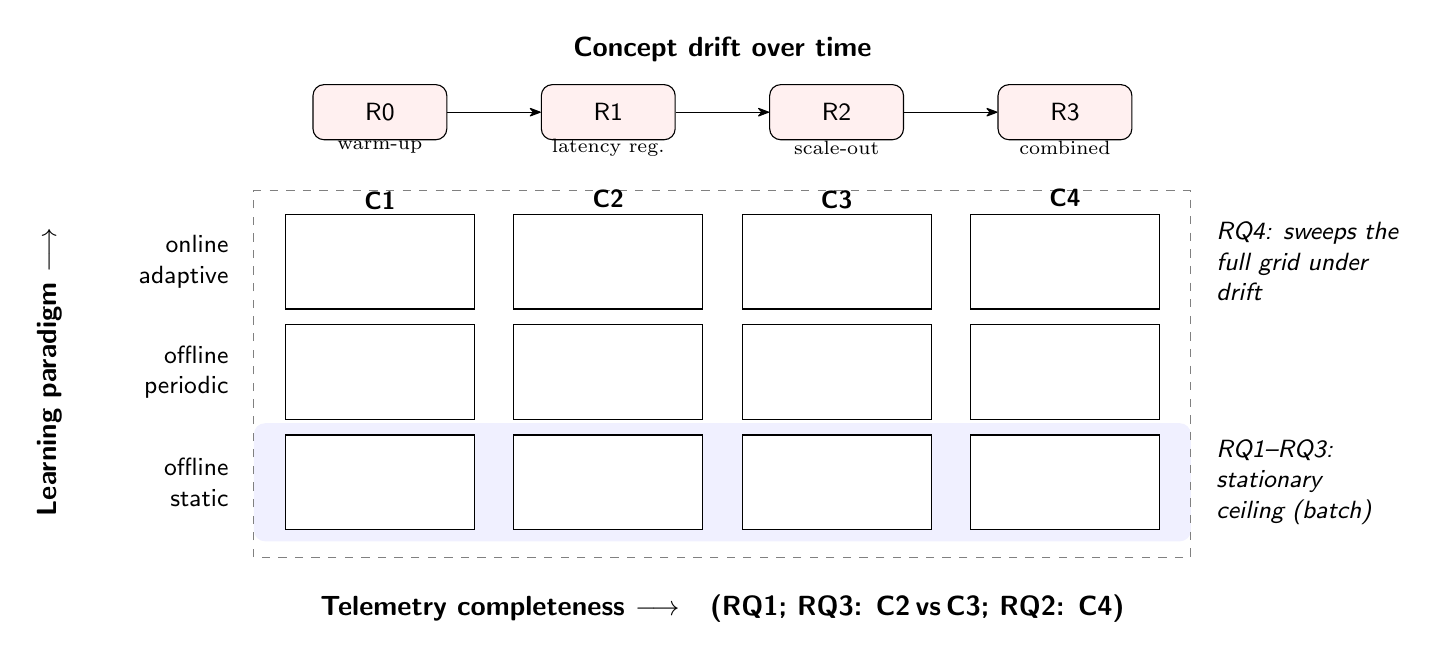
\begin{tikzpicture}[
  font=\sffamily\small,
  >={Stealth[round]},
  cell/.style={draw, minimum width=24mm, minimum height=12mm, align=center, inner sep=2pt, fill=white},
  hdr/.style={align=center, font=\sffamily\small\bfseries},
  rlab/.style={align=right, font=\sffamily\small},
  ann/.style={align=left, font=\sffamily\small\itshape},
]
% background: highlight static row + dashed grid box
\begin{scope}[on background layer]
  \fill[blue!6, rounded corners] (-1.6,-0.75) rectangle (10.3,0.75);
  \draw[dashed, gray] (-1.6,-0.95) rectangle (10.3,3.7);
\end{scope}
% drift timeline (top)
\node[font=\sffamily\bfseries] at (4.35,5.5) {Concept drift over time};
\foreach \r/\x/\s in {R0/0/warm-up, R1/2.9/{latency reg.}, R2/5.8/scale-out, R3/8.7/combined}{
  \node[draw, rounded corners, fill=red!6, minimum width=17mm, minimum height=7mm] (\r) at (\x,4.7) {\r};
  \node[font=\scriptsize] at (\x,4.25) {\s};
}
\draw[->] (R0) -- (R1); \draw[->] (R1) -- (R2); \draw[->] (R2) -- (R3);
% column headers
\foreach \c/\x/\sub in {C1/0/{Metrics}, C2/2.9/{{+}Logs}, C3/5.8/{{+}Traces}, C4/8.7/{{+}Events/hist.}}{\node[hdr] at (\x,3.4) {\c\\[-1pt]\footnotesize\sub};}
% cells
\foreach \rn/\ry in {online/2.8, periodic/1.4, static/0}{
  \foreach \cn/\cx in {C1/0,C2/2.9,C3/5.8,C4/8.7}{\node[cell] (\rn-\cn) at (\cx,\ry) {};}
}
% row labels (left, right-aligned outside the grid)
\node[rlab, anchor=east] at (-1.8,2.8) {online\\adaptive};
\node[rlab, anchor=east] at (-1.8,1.4) {offline\\periodic};
\node[rlab, anchor=east] at (-1.8,0) {offline\\static};
% right-side region annotations
\node[ann, anchor=west] at (10.5,2.8) {RQ4: sweeps the\\full grid under\\drift};
\node[ann, anchor=west] at (10.5,0) {RQ1--RQ3:\\stationary\\ceiling (batch)};
% axis labels
\node[font=\sffamily\bfseries] at (4.35,-1.6) {Telemetry completeness $\longrightarrow$\quad(RQ1; RQ3: C2\,vs\,C3; RQ2: C4)};
\node[font=\sffamily\bfseries, rotate=90] at (-4.2,1.4) {Learning paradigm $\longrightarrow$};
\end{tikzpicture}}
\caption{The two-axis experimental design. The identical pipeline is evaluated over
a grid of \emph{telemetry completeness} (C1--C4, horizontal; each a superset of the
previous) and \emph{learning paradigm} (static / periodic / online, vertical).
RQ1--RQ3 characterise the stationary ceiling on the batch (static) row; RQ4 sweeps
the whole grid on the drifted stream as the regimes $R_0\!\rightarrow\!R_3$ shift the
distribution.}\label{fig:design}
\end{figure} Because the feature extractor $\phi_c$, the fault schedule, the load profile and the seed are identical across all cells, any difference in outcome is attributable to the cell's coordinates---$(c, \pi)$---and not to a confound. This is the property that licenses the central claim: that the \emph{reversal} between the stationary ranking (RQ1) and the drifted ranking (RQ4) is caused by drift interacting with the learning policy, not by an incidental change of data or model.

%%===========================================================%%
\section{Methodology}\label{sec:method}
%%===========================================================%%

\subsection{Research design and philosophy}\label{sec:method-design}

The study adopts a positivist, deductive stance realised as a controlled, repeated-measures experiment, consistent with empirical software engineering. The relationships of interest are causal and comparative (``does \emph{X} affect detection?''), so the design isolates each independent variable while holding confounds constant. Two factors are manipulated---telemetry completeness $c$ and learning policy $\pi$---and the dependent variables are the detection-quality and operational-cost metrics of \S\ref{sec:method-metrics}. The control variables (model architecture, feature preprocessing, fault scenarios, load profile, random seed) are fixed across cells so that identical episodes are observed under differing configurations and policies. This within-subjects design is deliberate: because every cell sees the same underlying faults and the same drift schedule, differences cannot be ascribed to sampling variation between scenario sets.

\subsection{The TraceFlix testbed}\label{sec:method-testbed}

The platform is \emph{TraceFlix}, a Kubernetes microservice application representing a realistic cloud-native system. The mesh comprises three instrumented services with a genuine multi-hop dependency structure: \texttt{movie-service} issues $N$ sequential calls to \texttt{actor-service} and a call to \texttt{review-service}, so that a request traverses a caller/callee chain with realistic propagation. A three-service topology is chosen deliberately to keep fault attribution unambiguous and the controlled drift experiments tractable; the dependency chain is sufficient to exercise cross-service signal propagation for the localisation task, while remaining small enough that ground truth is never in doubt.

Instrumentation is end-to-end and vendor-neutral, matching what a production OpenTelemetry deployment emits, which maximises the external validity of the telemetry schema \cite{boten2022,hrusto2026}:
\begin{itemize}
  \item \textbf{Prometheus} --- metrics: CPU, memory, network, request latency, error rates and custom application counters.
  \item \textbf{Loki} --- structured application logs, container logs and Kubernetes event logs.
  \item \textbf{Tempo} --- OpenTelemetry-instrumented distributed traces of service-to-service calls.
  \item \textbf{Kubernetes events} --- OOMKilled and CrashLoopBackOff signals, the ``E'' of MELT.
  \item \textbf{Streaming transport} --- a message queue carries telemetry from TraceFlix to the detection pipeline for the online experiments.
\end{itemize}

Figure~\ref{fig:arch} shows the end-to-end testbed, organised as the canonical
observability stack \cite{kosinska2023}: an instrumented application emits
telemetry, a vendor-neutral collector normalises it, per-pillar backends store it,
and the detection pipeline consumes it. The four MELT pillars map directly onto the
four telemetry configurations of \S\ref{sec:method-configs}.

\begin{figure}[t]
\centering
\resizebox{\linewidth}{!}{%
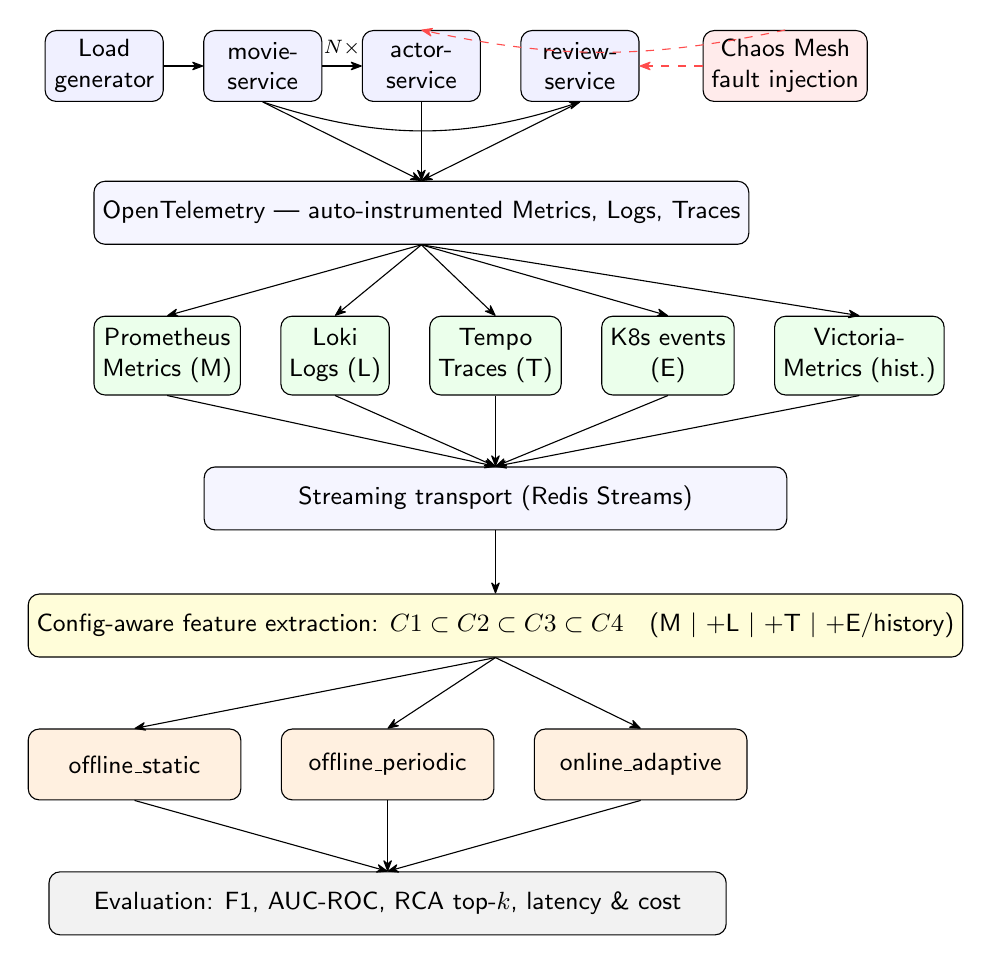
\begin{tikzpicture}[
  font=\sffamily\small,
  >={Stealth[round]},
  node distance=4mm and 5mm,
  svc/.style={draw, rounded corners, fill=blue!6, align=center, minimum height=9mm, minimum width=15mm, inner sep=3pt},
  bk/.style={draw, rounded corners, fill=green!8, align=center, minimum height=10mm, inner sep=3pt},
  wide/.style={draw, rounded corners, align=center, minimum height=8mm, inner sep=3pt},
  fault/.style={draw, rounded corners, fill=red!8, align=center, minimum height=9mm, inner sep=3pt},
  det/.style={draw, rounded corners, fill=orange!12, align=center, minimum height=9mm, minimum width=27mm, inner sep=3pt},
]
% Application row
\node[svc] (load) {Load\\generator};
\node[svc, right=of load] (movie) {movie-\\service};
\node[svc, right=of movie] (actor) {actor-\\service};
\node[svc, right=of actor] (review) {review-\\service};
\node[fault, right=8mm of review] (chaos) {Chaos Mesh\\fault injection};
\draw[->] (load) -- (movie);
\draw[->] (movie) -- node[above,font=\scriptsize]{$N\times$} (actor);
\draw[->] (movie.south) to[bend right=18] (review.south);
\draw[->, red!70, dashed] (chaos) -- (review);
\draw[->, red!70, dashed] (chaos.north) to[bend left=12] (actor.north);
% Instrumentation
\node[wide, fill=blue!4, below=10mm of actor, minimum width=74mm] (otel) {OpenTelemetry --- auto-instrumented Metrics, Logs, Traces};
\draw[->] (movie.south) -- (otel.north);
\draw[->] (actor.south) -- (otel.north);
\draw[->] (review.south) -- (otel.north);
% Backends
\node[bk, below=9mm of otel.south west, anchor=north west] (prom) {Prometheus\\Metrics (M)};
\node[bk, right=of prom] (loki) {Loki\\Logs (L)};
\node[bk, right=of loki] (tempo) {Tempo\\Traces (T)};
\node[bk, right=of tempo] (events) {K8s events\\(E)};
\node[bk, right=of events] (vm) {Victoria-\\Metrics (hist.)};
\foreach \b in {prom,loki,tempo,events,vm} {\draw[->] (otel.south) -- (\b.north);}
% Transport
\node[wide, fill=blue!4, below=9mm of tempo, minimum width=74mm] (stream) {Streaming transport (Redis Streams)};
\foreach \b in {prom,loki,tempo,events,vm} {\draw[->] (\b.south) -- (stream.north);}
% Feature extraction
\node[wide, fill=yellow!15, below=8mm of stream, minimum width=86mm] (feat) {Config-aware feature extraction: $C1 \subset C2 \subset C3 \subset C4$\quad(M $\mid$ {+}L $\mid$ {+}T $\mid$ {+}E/history)};
\draw[->] (stream) -- (feat);
% Detectors
\node[det, below=9mm of feat.south west, anchor=north west] (d1) {offline\_static};
\node[det, right=of d1] (d2) {offline\_periodic};
\node[det, right=of d2] (d3) {online\_adaptive};
\foreach \d in {d1,d2,d3} {\draw[->] (feat.south) -- (\d.north);}
% Evaluation
\node[wide, fill=gray!10, below=9mm of d2, minimum width=86mm] (eval) {Evaluation: F1, AUC-ROC, RCA top-$k$, latency \& cost};
\foreach \d in {d1,d2,d3} {\draw[->] (\d.south) -- (eval.north);}
\end{tikzpicture}}
\caption{The TraceFlix testbed and detection pipeline. A load generator drives the
instrumented microservice mesh (\texttt{movie}$\rightarrow$\texttt{actor}$\times N$,
\texttt{movie}$\rightarrow$\texttt{review}); Chaos Mesh injects timestamped faults.
OpenTelemetry collects MELT telemetry into per-pillar backends, whose signals are
streamed to a configuration-aware feature extractor (C1--C4) feeding the three
learning policies and the evaluation harness.}\label{fig:arch}
\end{figure}

\subsection{Fault injection and ground-truth labelling}\label{sec:method-faults}

Ground-truth labels are generated by controlled fault injection following the timestamped-injection methodology of Pedroso et al.\ \cite{pedroso2025}. Faults are applied to running pods with precise start/stop timestamps, which become the labels against which detector output is scored. The fault taxonomy spans resource-exhaustion, performance-degradation and availability modes: memory leaks, CPU saturation, latency spikes, error bursts, OOMKilled events, CrashLoopBackOff, connection-pool exhaustion and network partitions. To produce genuine Kubernetes events for the ``E'' signal used by C4, container resource limits are patched so that memory-leak faults escalate to real OOMKills rather than simulated ones. A load generator drives continuous, realistic traffic so that each fault rides on a live request stream rather than an idle system; each \emph{episode} selects a service as the fault origin, applies the fault, and lets dependent services exhibit secondary effects (e.g.\ induced latency), reproducing realistic fault propagation for RCA.

\subsection{Telemetry configurations (the completeness axis)}\label{sec:method-configs}

The completeness axis is operationalised as four ordered, nested configurations (Table~\ref{tab:configs}). Feature engineering is \emph{configuration-aware}: only the feature families permitted by the active configuration are assembled, so an identical telemetry window yields different feature vectors per configuration. This is the mechanism that isolates signal availability as the independent variable.

\begin{table}[t]
\caption{The four telemetry configurations (completeness axis). Each is a strict superset of the previous, enabling marginal-contribution analysis.}\label{tab:configs}
\begin{tabular}{@{}llcl@{}}
\toprule
Config & Signals & Features & Represents \\
\midrule
C1 & Metrics only        & 10 & Basic infrastructure monitoring \\
C2 & Metrics ${+}$ Logs  & 14 & Intermediate observability \\
C3 & ${+}$ Traces        & 18 & Full three-pillar observability \\
C4 & Full MELT (${+}$ Events ${+}$ history) & 23 & Advanced observability \\
\bottomrule
\end{tabular}
\end{table}

Feature engineering operates on the telemetry falling within each fixed-length window and aggregates it into a flat vector, so that all model families consume a common tabular representation. The feature families added by each pillar are summarised in Table~\ref{tab:features} (the full per-feature listing is given in Appendix~\ref{app:features}). The metrics pillar (C1) contributes per-window aggregates of resource and request signals---CPU and memory utilisation, request and error rates, and latency percentiles---which are the signals available to any team with basic monitoring. Logs (C2) add volume- and severity-based features (error- and warning-log counts and a log-template diversity measure) that disambiguate anomalies whose metric signature is equivocal. Traces (C3) add span-level features---span rate, mean span duration, error-span rate---and, critically for localisation, the \emph{originating-error-span} feature that identifies the service at which an error tree begins rather than the services that merely propagate its latency. Events and history (C4) add Kubernetes lifecycle-event counts (OOMKilled, CrashLoopBackOff, restarts) and rolling-baseline deviation features that encode how far the current window departs from a longer historical norm.

\begin{table}[t]
\caption{Feature families added by each pillar. Counts are cumulative across the nested configurations (cf.\ Appendix~\ref{app:features}).}\label{tab:features}
\begin{tabular}{@{}llcp{0.44\textwidth}@{}}
\toprule
Pillar & Added at & ${+}$Feat. & Representative features \\
\midrule
Metrics & C1 & 10 & CPU/mem util., req.\ rate, error rate, p50/p95/p99 latency, net I/O, restarts \\
Logs    & C2 & 4  & log volume, error-log count, warn-log count, template diversity \\
Traces  & C3 & 4  & span rate, mean span duration, error-span rate, originating-error-span \\
Events${+}$history & C4 & 5 & OOMKilled, CrashLoopBackOff, restart events, rolling-baseline deviations \\
\bottomrule
\end{tabular}
\end{table}

Two properties of this design matter for the validity of the completeness comparison. First, the feature families are \emph{additive and disjoint}: enabling a pillar adds its features without altering those of lower pillars, so an identical telemetry window produces feature vectors that are strict prefixes of one another as $c$ increases. Second, all features are window-local aggregates, deliberately avoiding high-cardinality raw identifiers (\S\ref{sec:bg-tooling}); this keeps the representation production-realistic and ensures the online model's per-window update cost is bounded by a small, fixed dimensionality rather than growing with traffic.

\subsection{Drift regimes (the temporal axis)}\label{sec:method-regimes}

Non-stationarity is induced as a controlled sequence of operating regimes, each representing a common operational event that shifts the telemetry distribution:
\begin{description}
  \item[$R_0$ --- Baseline.] The nominal operating point; the offline models train here.
  \item[$R_1$ --- Latency regression.] A deployment-style shift that raises baseline service latency, moving the ``normal'' latency distribution.
  \item[$R_2$ --- Scale-out.] An autoscaling event that changes replica counts and therefore per-pod resource-utilisation baselines.
  \item[$R_3$ --- Combined load.] A traffic surge superimposed on the previous shifts---the hardest, most-drifted regime, moving multiple distributions at once.
\end{description}
The stream is processed prequentially over $320$ episodes and $11{,}520$ windows, of which $2{,}880$ constitute the $R_0$ warm-up and $8{,}640$ the drifted future ($R_1$--$R_3$) on which RQ4 is scored.

\subsection{Learners and the online model}\label{sec:method-learners}

Four learners instantiate the temporal axis (Table~\ref{tab:learners}). The offline learners use a Random Forest, chosen because RQ2 (\S\ref{sec:res-rq2}) identifies ensemble trees as the strongest family on this multimodal tabular telemetry. The online learner is a streaming model built for prequential operation.

\begin{table}[t]
\caption{Learners instantiating the temporal axis.}\label{tab:learners}
\begin{tabular}{@{}llp{0.42\textwidth}@{}}
\toprule
Learner & Family & Learning policy \\
\midrule
\texttt{offline\_static}   & Random Forest & Train once on $R_0$, then frozen \\
\texttt{offline\_periodic} & Random Forest & Refit every $500$ windows on a $2{,}880$-window buffer \\
\texttt{online\_adaptive}  & SGD ${+}$ adaptive norm. ${+}$ bandit & Prequential \texttt{partial\_fit}, one window at a time \\
\texttt{offline\_full}     & Random Forest & Oracle: trained on all regimes (reference ceiling) \\
\bottomrule
\end{tabular}
\end{table}

The online detector combines three mechanisms designed to track drift without retaining history (Algorithm~\ref{alg:online}). First, an incrementally-fitted linear classifier (stochastic gradient descent, logistic loss) updates on every window. Second, an exponentially-weighted (EW) running normaliser rescales each feature using running estimates of its mean and variance, so that a shift in a feature's baseline---the signature of drift---is absorbed by the normaliser rather than corrupting the decision boundary. Third, a \emph{champion bandit} maintains a small pool of candidate learning-rate/regularisation configurations and re-selects the current champion by recent prequential F1 whenever a candidate overtakes the incumbent, providing drift-triggered adaptation of the update dynamics themselves.

\begin{algorithm}[t]
\caption{Online-adaptive prequential detection}\label{alg:online}
\begin{algorithmic}[1]
\State \textbf{Input:} telemetry stream; candidate set $\mathcal{H}=\{(\eta_0,\alpha)\}$
\State Initialise EW normaliser $\mathcal{N}$; models $\{m_h\}_{h\in\mathcal{H}}$; champion $h^\star \gets$ default
\For{each window $t = 1, 2, \dots$}
  \State $\mathbf{x}_t \gets \phi_c(\text{telemetry}_t)$ \Comment{configuration-aware features}
  \State $\tilde{\mathbf{x}}_t \gets \mathcal{N}.\textsc{transform}(\mathbf{x}_t)$ \Comment{rescale by running mean/var}
  \State $\hat{y}_t \gets m_{h^\star}.\textsc{predict}(\tilde{\mathbf{x}}_t)$ \Comment{test before train}
  \State \textbf{emit} $\hat{y}_t$
  \State observe label $y_t$
  \State $\mathcal{N}.\textsc{update}(\mathbf{x}_t)$
  \For{$h \in \mathcal{H}$} \Comment{update all candidates}
     \State $m_h.\textsc{partial\_fit}(\tilde{\mathbf{x}}_t, y_t)$
     \State update rolling prequential F1 of $m_h$
  \EndFor
  \If{$\arg\max_h \text{F1}(m_h) \neq h^\star$} \Comment{drift-triggered re-selection}
     \State $h^\star \gets \arg\max_h \text{F1}(m_h)$; record adapt event
  \EndIf
\EndFor
\end{algorithmic}
\end{algorithm}

The three mechanisms have the following precise form. The classifier maintains a weight vector $\mathbf{w}$ updated by stochastic gradient descent on the logistic loss with $\ell_2$ regularisation strength $\alpha$ and an inverse-scaling learning rate derived from $\eta_0$; the per-window update touches only the $d_c$ active weights and is therefore $O(d_c)$ in both time and memory, with no dependence on stream length. The exponentially-weighted normaliser maintains, for each feature $j$, running estimates updated at every window with decay $\lambda$,
\begin{align}
  \mu_{t,j} &= (1-\lambda)\,\mu_{t-1,j} + \lambda\, x_{t,j}, \\
  s^2_{t,j} &= (1-\lambda)\,s^2_{t-1,j} + \lambda\,(x_{t,j}-\mu_{t,j})^2,
\end{align}
and rescales the input as $\tilde{x}_{t,j} = (x_{t,j}-\mu_{t,j})/\sqrt{s^2_{t,j}+\varepsilon}$. Because $\mu$ and $s^2$ track the moving feature distribution, a virtual-drift shift in a feature's baseline (\S\ref{sec:prob-drift}) is absorbed into the normaliser rather than presented to the classifier as a spurious anomaly---this is the mechanism that protects against the stale-normal precision collapse. The champion bandit maintains the candidate pool $\mathcal{H} = \{\,(\eta_0,\alpha) : \eta_0 \in \{0.01,0.05,0.1\},\ \alpha \in \{10^{-4},10^{-3}\}\,\}$, scores each candidate by its prequential F1 over a trailing window, and re-selects the champion $h^\star$ only when a challenger exceeds the incumbent by a margin $\delta$, a hysteresis that prevents thrashing between near-tied candidates. Re-selection events are logged as ``adapt events'' and reported in \S\ref{sec:res-rq4-adapt}; their frequency is itself an indicator of how hard the drift is to track at a given telemetry richness.

For RQ2 the model-family comparison additionally evaluates, on the richest configuration C4, Random Forest, two gradient-boosting implementations, an LSTM temporal model, and an attention-style late-fusion model drawing on the building-blocks strategy of HolisticRCA \cite{han2024}. For RQ3 the localisation component ranks candidate fault entities, comparing a metrics-and-logs localiser (C2 features) against one that additionally consumes the trace-derived originating-error-span signal (C3 features), thereby isolating the marginal RCA value of tracing.

\subsection{Evaluation and cost metrics}\label{sec:method-metrics}

Detection is evaluated with precision, recall, F1 and AUC-ROC. F1 is the headline metric because anomaly data are class-imbalanced (normal windows dominate), under which raw accuracy is misleading---a trivial always-normal predictor scores high on accuracy but has zero recall. For the streaming experiments, F1 is computed \emph{prequentially} over the future ($R_1$--$R_3$) windows. Root-cause localisation is measured by top-$k$ accuracy; on a three-service topology top-2 saturates near unity, so \textbf{top-1 is the discriminating metric}.

Because RQ4 reframes the choice of paradigm as an operational decision, we additionally report operational-cost metrics that a static accuracy comparison omits: \emph{maximum per-window latency} (the tail cost, which exposes retraining spikes), \emph{model footprint} in kilobytes, the number of \emph{retained historical windows} (a data-governance and memory cost), and \emph{total CPU time}. These let us characterise the accuracy/cost trade-off rather than accuracy alone.

\subsection{Reproducibility}\label{sec:method-repro}

All models are trained and evaluated under a fixed random seed, an identical train/test protocol and the same preprocessing, so cross-cell differences reflect configuration and policy rather than stochastic training variation. The synthetic prequential stream is generated deterministically. All tooling is open-source, and the result datasets (\texttt{rq1\_completeness}, \texttt{rq3\_rca}, \texttt{rq4\_online\_vs\_offline}, \texttt{rq4\_cost}, \texttt{rq4\_timeline} and their summaries) underpin every figure and table reported below.

\subsection{Threats to validity}\label{sec:method-threats}

\paragraph{Internal validity.} Held-constant controls (model, seed, scenarios, load) and the nested within-subjects design mean cross-cell differences are attributable to the manipulated factors. Fault-injection timing jitter could blur labels; this is mitigated by recording exact start/stop timestamps.

\paragraph{External validity.} A testbed cannot reproduce the full heterogeneity of production \cite{hrusto2026}. This is mitigated by real OpenTelemetry instrumentation and unmodified backends (so the telemetry schema is production-representative) and by a fault taxonomy drawn from documented real-world failure modes. The three-service topology limits topological generalisation, an acknowledged boundary condition; and the RQ4 stream, while drift-controlled, is synthetic-prequential, so absolute F1 values are testbed-specific even though the \emph{ordering} of paradigms is the result of interest.

\paragraph{Construct validity.} ``Detection effectiveness'' is multidimensional; using F1, AUC-ROC, latency and cost together avoids over-reliance on a single construct.

\paragraph{Conclusion validity.} A fixed seed and a within-subjects design across all $(c,\pi)$ cells guard against over-interpreting noise; the RQ4 effect sizes (\S\ref{sec:res-rq4}) are large relative to any plausible residual variance.

%%===========================================================%%
\section{Results}\label{sec:results}
%%===========================================================%%

We first establish the stationary ceiling along the completeness axis (RQ1--RQ3), then turn to the headline drift comparison (RQ4).

\subsection{RQ1 --- The completeness ceiling}\label{sec:res-rq1}

Table~\ref{tab:rq1} reports single-pass detection on the stationary held-out set for the best batch model at each configuration. The result is unambiguous: detection quality rises \emph{monotonically} with telemetry richness, F1 climbing from $0.906$ (metrics-only) to $0.994$ (full MELT)---a reduction of the error complement from roughly nine per cent to under one per cent.

\begin{table}[t]
\caption{RQ1 --- stationary detection by configuration (best batch model). Higher is better.}\label{tab:rq1}
\begin{tabular}{@{}llccccc@{}}
\toprule
Config & Name & Feat. & Precision & Recall & F1 & AUC-ROC \\
\midrule
C1 & Metrics-Only            & 10 & 0.9509 & 0.8659 & 0.9064 & 0.9740 \\
C2 & Metrics${+}$Logs        & 14 & 0.9601 & 0.9078 & 0.9332 & 0.9847 \\
C3 & ${+}$Traces             & 18 & 0.9847 & 0.9916 & 0.9882 & 0.9994 \\
C4 & Full MELT               & 23 & 0.9944 & 0.9930 & \textbf{0.9937} & 0.9993 \\
\bottomrule
\end{tabular}
\end{table}

\begin{figure}[t]
\centering
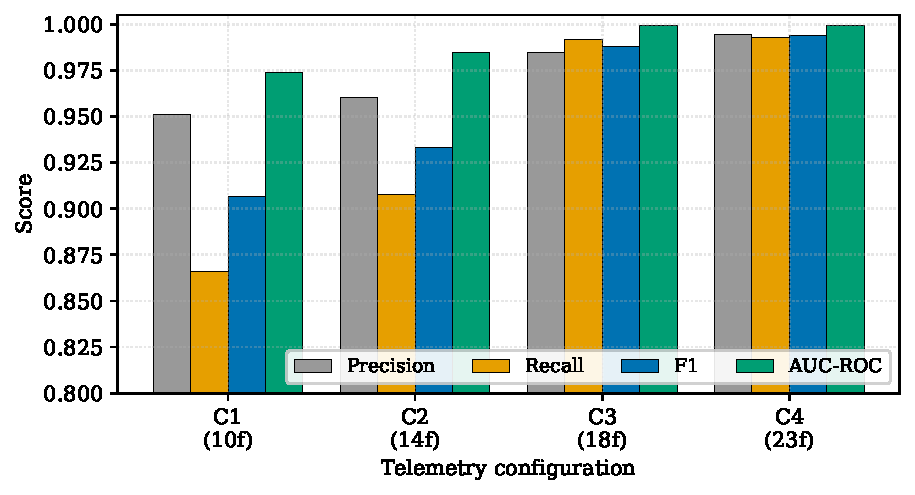
\includegraphics[width=0.86\textwidth]{fig_rq1_completeness.pdf}
\caption{RQ1 --- stationary detection quality across the four telemetry configurations (best batch model). All four metrics improve as completeness increases; the largest single jump is the addition of traces (C2$\rightarrow$C3).}\label{fig:rq1}
\end{figure}

The pattern of increments is itself informative. Adding logs (C1$\rightarrow$C2) yields a moderate F1 gain of $\sim 2.7$ points, driven principally by recall as log-based error signals disambiguate anomalies whose metric signature alone was equivocal. Adding \emph{traces} (C2$\rightarrow$C3) yields a markedly larger gain of $\sim 5.5$ points, lifting both precision and recall above $0.99$: traces resolve the cross-service signal that metrics and logs miss. Adding events and history (C3$\rightarrow$C4) yields only a marginal further gain, the two richest configurations being effectively indistinguishable on detection. Two conclusions follow. First, the single most valuable increment for \emph{detection} on this testbed is distributed traces---a more specific finding than the literature's general ``more is better'' \cite{lomio2022,han2024}. Second, the near-equivalence of C3 and C4 suggests that for detection the three classical pillars already capture almost all available signal, and the marginal value of events lies elsewhere (localisation and, as RQ4 shows, the cost of adaptation). \textbf{This is the stationary ceiling; RQ4 shows what happens to it once the stream drifts.}

\subsection{RQ2 --- Model families}\label{sec:res-rq2}

Table~\ref{tab:rq2} compares five model families on the richest configuration (C4) with identical inputs. Ensemble trees are the most effective family: Random Forest attains the highest F1 ($0.9937$), closely followed by the two gradient-boosting implementations, all three exceeding $0.99$ precision---few false alarms, an operationally desirable property given the cost of alert fatigue. The temporal (LSTM) and late-fusion models underperform, instructively rather than disappointingly: the windowed feature representation already captures much per-window signal, leaving less for a temporal model to exploit, and the late-fusion architecture's requirement of cross-pillar agreement suppresses false positives at the cost of recall.

\begin{table}[t]
\caption{RQ2 --- detection by model family on full MELT (C4). Ensemble trees lead.}\label{tab:rq2}
\begin{tabular}{@{}lcccc@{}}
\toprule
Model family & Precision & Recall & F1 & Note \\
\midrule
Random Forest        & 0.994 & 0.993 & \textbf{0.994} & best overall \\
Gradient Boosting A  & 0.993 & 0.989 & 0.991 & close second \\
Gradient Boosting B  & 0.992 & 0.987 & 0.989 & close third \\
Late fusion          & 0.991 & 0.872 & 0.928 & high prec., low recall \\
LSTM (temporal)      & 0.910 & 0.781 & 0.841 & fallback path \\
\bottomrule
\end{tabular}
\end{table}

The lesson, which directly informs RQ4, is that the benefit of rich multimodal data is conditioned on the model's capacity to exploit it: a powerful, data-hungry architecture does not automatically beat a simpler ensemble when the feature representation is already informative. This is why the offline learners in RQ4 use a Random Forest, and why the online learner is a lightweight linear model---on tabular telemetry, simplicity buys both accuracy and the cheap, bounded per-window update that streaming requires.

This raises an apparent tension that is worth confronting directly: if ensemble trees are the strongest \emph{batch} family (RQ2), why is the \emph{online} learner not also a tree? The answer is that the two settings reward different properties. A Random Forest is an excellent \emph{static} estimator but a poor \emph{incremental} one: it cannot be updated by a single example without either refitting (the expensive, bursty periodic path) or resorting to incremental-tree variants whose drift behaviour in the upper splits is fragile. The online setting prizes a bounded, smooth per-window update and graceful adaptation over raw stationary accuracy, and a normalised linear model delivers exactly that---its per-update cost is $O(d_c)$, its footprint is kilobytes, and, crucially, the configuration-aware features (\S\ref{sec:method-configs}) have already done the non-linear work of summarising raw telemetry into informative aggregates, leaving a decision surface that is close to linearly separable. The RQ4 results vindicate the choice: the linear online model not only beats both batch paradigms on the drifted stream but, under full telemetry, exceeds the Random-Forest oracle itself (Table~\ref{tab:rq4-head}). The strongest \emph{static} model and the strongest \emph{streaming} model are simply not the same model, and conflating the two is one way the single-snapshot literature is misled.

\subsection{RQ3 --- Trace-driven localisation}\label{sec:res-rq3}

Table~\ref{tab:rq3} reports root-cause localisation with traces excluded (C2) versus included (C3). The introduction of traces raises top-1 accuracy from $0.9068$ to a perfect $1.0000$, eliminating the localisation errors the metric-and-log approach commits.

\begin{table}[t]
\caption{RQ3 --- root-cause localisation, traces excluded vs.\ included. Top-1 is the discriminating metric on a three-service topology.}\label{tab:rq3}
\begin{tabular}{@{}lcc@{}}
\toprule
Approach & top-1 accuracy & top-2 accuracy \\
\midrule
Metrics${+}$Logs (C2)            & 0.9068 & 1.0000 \\
Metrics${+}$Logs${+}$Traces (C3) & \textbf{1.0000} & 1.0000 \\
\bottomrule
\end{tabular}
\end{table}

The mechanism, as anticipated in the design, lies in the originating-error-span feature. Under the metric-and-log approach a downstream fault raises the latency of the services that depend on it, so the anomaly score implicates dependents almost as strongly as the true culprit; where the secondary symptom is pronounced, a dependent service is ranked first and localisation fails. The trace feature resolves the ambiguity: only the originating service accumulates originating error spans, pulling the true root cause unambiguously to the top. Top-2 saturates at unity even without traces---on three services it covers two-thirds of the mesh and is therefore uninformative---which is why top-1 is the discriminating measure. This is precisely the controlled, ablation-style evidence the literature was shown to lack: where Han et al.\ \cite{han2024} demonstrate that a fused multimodal architecture beats single-modal baselines, we isolate the trace modality and quantify its marginal contribution while holding all else constant.

\subsection{RQ4 --- Learning under drift}\label{sec:res-rq4}

RQ1--RQ3 measured a \emph{stationary} ceiling. We now re-use the identical pipeline and feature sets on the drifted future stream ($8{,}640$ post-warm-up windows across $R_1$--$R_3$) and compare the three realisable learning policies, with the all-regimes oracle as a ceiling.

\subsubsection{Headline: F1 on the drifted stream}\label{sec:res-rq4-head}

Table~\ref{tab:rq4-head} and Fig.~\ref{fig:rq4head} report F1 over the future stream. The result inverts the stationary picture. The frozen batch model collapses to F1 $\approx 0.49$--$0.51$ \emph{regardless} of how much telemetry it is given: going from metrics-only to full MELT moves its F1 by barely two points ($0.4894 \rightarrow 0.5112$). Scheduled retraining recovers substantially (up to $\sim 0.89$) but always trails. The online-adaptive model \emph{wins at every configuration}, reaching $0.9817$ under C3 and $0.9834$ under C4---and, notably, exceeding the all-regimes oracle ($0.9387$ at C4; Table~\ref{tab:rq4-regime} note), because the oracle still fits a single static boundary across all regimes whereas the online model tracks each regime as it arrives.

\begin{table}[t]
\caption{RQ4 headline --- F1 on the future (drifted) stream. Best realisable learner in bold.}\label{tab:rq4-head}
\begin{tabular}{@{}lccccc@{}}
\toprule
Config & static & periodic & online & gain vs.\ static & gain vs.\ periodic \\
\midrule
C1 Metrics-Only        & 0.4894 & 0.7574 & \textbf{0.8174} & $+0.3280$ & $+0.0600$ \\
C2 Metrics${+}$Logs    & 0.4921 & 0.7776 & \textbf{0.8347} & $+0.3426$ & $+0.0571$ \\
C3 ${+}$Traces         & 0.5097 & 0.8904 & \textbf{0.9817} & $+0.4720$ & $+0.0913$ \\
C4 Full MELT           & 0.5112 & 0.8905 & \textbf{0.9834} & $+0.4722$ & $+0.0929$ \\
\bottomrule
\end{tabular}
\end{table}

\begin{figure}[t]
\centering
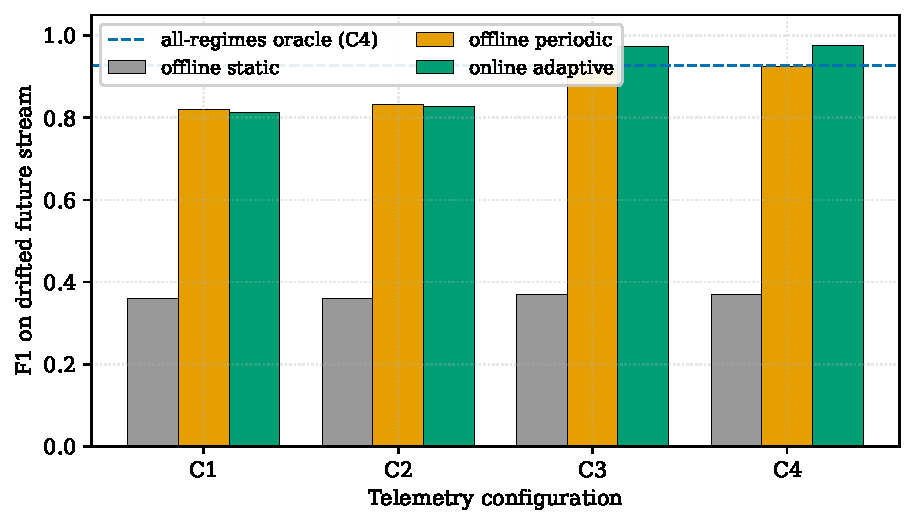
\includegraphics[width=0.86\textwidth]{fig_rq3_headline.pdf}
\caption{RQ4 headline --- F1 on the drifted future stream by learning policy and configuration. The frozen static model (grey) is flat and low regardless of telemetry; periodic retraining (orange) recovers partially; the online-adaptive model (green) dominates everywhere and, under C3/C4, exceeds the all-regimes oracle (dashed). Contrast with the monotonic stationary ceiling of Fig.~\ref{fig:rq1}.}\label{fig:rq4head}
\end{figure}

Two features deserve emphasis. First, telemetry richness barely helps the \emph{static} model (the $+0.02$ from C1 to C4 is within noise) but strongly helps the \emph{online} model (the $+0.17$ from C1 to C4 closes almost the entire gap to the ceiling). Completeness and adaptation are thus \emph{complementary}: richer signal raises the attainable ceiling, but only adaptation realises it. Second, the online model's gain over periodic retraining \emph{widens} with richness ($+0.060$ at C1 to $+0.093$ at C4): the more informative the features, the more a continuous learner can extract from each window relative to a lagging batch refit.

\subsubsection{Precision, recall and the stale-normal signature}\label{sec:res-rq4-prf}

The F1 headline conceals \emph{how} each policy fails, which Table~\ref{tab:rq4-prf} makes explicit by decomposing the future-stream score into precision, recall and AUC-ROC. The static model exhibits the stale-normal signature in its purest form: its recall is near-perfect ($0.97$--$1.00$) while its precision collapses to $0.33$--$0.34$ at every configuration. That combination is diagnostic---the frozen boundary still fires on the genuine anomalies (high recall) but, because the post-drift normal has moved into the region it labels anomalous, it also fires on healthy traffic, so the overwhelming majority of its alerts are false. No amount of additional telemetry corrects this: the precision is flat across C1--C4 because the failure is in the boundary's \emph{location}, not in the features' \emph{informativeness}. The online model shows the opposite profile, trading a little recall for a large precision gain ($0.87$--$0.99$), which is the operationally desirable direction given the cost of alert fatigue.

\begin{table}[t]
\caption{RQ4 --- future-stream precision (P), recall (R) and AUC-ROC by policy and configuration. The static model's flat, collapsed precision with near-perfect recall is the stale-normal signature.}\label{tab:rq4-prf}
\begin{tabular}{@{}llccc@{}}
\toprule
Config & Policy & P & R & AUC \\
\midrule
\multirow{3}{*}{C1}
 & static   & 0.327 & 0.974 & 0.699 \\
 & periodic & 0.706 & 0.817 & 0.906 \\
 & online   & 0.868 & 0.773 & 0.934 \\
\midrule
\multirow{3}{*}{C2}
 & static   & 0.329 & 0.980 & 0.700 \\
 & periodic & 0.716 & 0.851 & 0.919 \\
 & online   & 0.874 & 0.799 & 0.950 \\
\midrule
\multirow{3}{*}{C3}
 & static   & 0.342 & 0.999 & 0.874 \\
 & periodic & 0.821 & 0.973 & 0.979 \\
 & online   & 0.988 & 0.976 & 0.998 \\
\midrule
\multirow{3}{*}{C4}
 & static   & 0.343 & 1.000 & 0.886 \\
 & periodic & 0.822 & 0.972 & 0.980 \\
 & online   & 0.989 & 0.978 & 0.998 \\
\bottomrule
\end{tabular}
\end{table}

A subtler point hides in the AUC column. The static model's \emph{thresholded} F1 is flat across configurations, yet its AUC-ROC rises markedly with telemetry, from $0.70$ at C1 to $0.89$ at C4. This means richer telemetry does improve the static model's \emph{ranking} of windows by anomaly score---traces in particular make anomalous windows more separable---but that improvement is invisible at the fixed operating threshold, because the threshold itself is calibrated to a distribution that no longer holds. In other words, more telemetry sharpens the score but not the stale \emph{cut-point}; only re-learning moves the cut-point. This is a precise, quantitative statement of why completeness and adaptation are complementary rather than substitutable, and it is a distinction that an F1-only analysis would miss entirely.

\subsubsection{Per-regime breakdown}\label{sec:res-rq4-regime}

Table~\ref{tab:rq4-regime} decomposes F1 by regime, and the decomposition is more revealing than the headline. The online model is best in $10$ of the $12$ regime$\times$configuration cells; the two exceptions are both in the \emph{scale-out} regime ($R_2$) under the thinnest telemetry (C1 and C2), where periodic retraining narrowly leads. This exception is theoretically coherent rather than anomalous: scale-out is predominantly \emph{virtual} drift (\S\ref{sec:prob-drift})---the feature baselines shift but the meaning of ``anomalous'' does not---so a batch refit on recent data recovers the boundary as well as continuous updating, and with thin telemetry the online normaliser has fewer signals to re-centre. By contrast, $R_1$ \emph{latency regression} is \emph{real} concept drift, and it is there that the static model is hurt most (F1 $\approx 0.44$, its lowest), while the online model holds $0.83$--$0.99$. The static model's deficit is thus widest exactly where the drift is conceptual, not merely distributional---the classic stale-normal signature, visible as preserved recall ($\sim 0.97$--$1.00$) with collapsed precision ($\sim 0.33$--$0.34$).

\begin{table}[t]
\caption{RQ4 per-regime F1 by configuration. Best learner per cell in bold. (s = static, p = periodic, o = online.) The all-regimes oracle attains 0.812 (C1), 0.834 (C2), 0.940 (C3), 0.939 (C4); the online model exceeds it at C3--C4.}\label{tab:rq4-regime}
\begin{tabular}{@{}llccc@{}}
\toprule
Config & Regime & s & p & o \\
\midrule
\multirow{3}{*}{C1}
 & $R_1$ latency regression & 0.4446 & 0.6950 & \textbf{0.8294} \\
 & $R_2$ scale-out          & 0.5743 & \textbf{0.8003} & 0.7912 \\
 & $R_3$ combined load      & 0.4751 & 0.7942 & \textbf{0.8286} \\
\midrule
\multirow{3}{*}{C2}
 & $R_1$ latency regression & 0.4484 & 0.7131 & \textbf{0.8548} \\
 & $R_2$ scale-out          & 0.5797 & \textbf{0.8153} & 0.7997 \\
 & $R_3$ combined load      & 0.4750 & 0.8201 & \textbf{0.8458} \\
\midrule
\multirow{3}{*}{C3}
 & $R_1$ latency regression & 0.4351 & 0.7961 & \textbf{0.9858} \\
 & $R_2$ scale-out          & 0.6842 & 0.9610 & \textbf{0.9772} \\
 & $R_3$ combined load      & 0.4782 & 0.9310 & \textbf{0.9819} \\
\midrule
\multirow{3}{*}{C4}
 & $R_1$ latency regression & 0.4350 & 0.7942 & \textbf{0.9885} \\
 & $R_2$ scale-out          & 0.6939 & 0.9610 & \textbf{0.9793} \\
 & $R_3$ combined load      & 0.4778 & 0.9335 & \textbf{0.9825} \\
\bottomrule
\end{tabular}
\end{table}

\subsubsection{Operational cost}\label{sec:res-rq4-cost}

Detection quality is only half the decision. Table~\ref{tab:rq4-cost} compares the periodic and online learners on operational cost. The operational measurements (latency, footprint, retained windows, CPU) come from a dedicated cost-profiling run; because they reflect the \emph{mechanism} rather than the dataset size, they are reported alongside the Run-B headline F1 for a single consistent quality figure. The two paradigms have opposite cost profiles (Fig.~\ref{fig:rq4cost}). Periodic retraining produces large per-window \emph{tail} spikes---up to $\sim 650$ ms when a refit lands---$17$--$32\times$ worse than the online model's bounded per-window cost ($\leq 37$ ms). The online model is also $\sim 200$--$550\times$ smaller ($\approx 15$ KB versus $3$--$8$ MB) and retains \emph{zero} historical windows, against the $2{,}880$-window labelled buffer the periodic model must hold to refit. Its only disadvantage is aggregate CPU: because it updates on every future window rather than performing a handful of batch refits, it spends $\sim 4$--$6\times$ the periodic total---but spends it \emph{smoothly}, never stalling the pipeline with a multi-hundred-millisecond spike.

\begin{table}[t]
\caption{RQ4 cost --- periodic vs.\ online. Latency is the per-window maximum (tail); operational columns are from the cost-profiling run, F1 is the Run-B future-stream F1 of Table~\ref{tab:rq4-head}.}\label{tab:rq4-cost}
\begin{tabular}{@{}llccccc@{}}
\toprule
Config & Learner & F1 & Max ms/win & Size (KB) & Retained win. & Total s \\
\midrule
\multirow{2}{*}{C1} & periodic & 0.7574 & 621.0 & 8290.4 & 2880 & 6.48 \\
                    & online   & 0.8174 & 31.3  & 14.9   & 0    & 36.72 \\
\midrule
\multirow{2}{*}{C2} & periodic & 0.7776 & 621.4 & 7979.2 & 2880 & 6.50 \\
                    & online   & 0.8347 & 36.9  & 15.2   & 0    & 37.86 \\
\midrule
\multirow{2}{*}{C3} & periodic & 0.8904 & 646.5 & 3047.0 & 2880 & 6.52 \\
                    & online   & 0.9817 & 28.7  & 15.4   & 0    & 36.87 \\
\midrule
\multirow{2}{*}{C4} & periodic & 0.8905 & 594.0 & 3588.8 & 2880 & 6.28 \\
                    & online   & 0.9834 & 18.9  & 15.7   & 0    & 27.60 \\
\bottomrule
\end{tabular}
\end{table}

\begin{figure}[t]
\centering
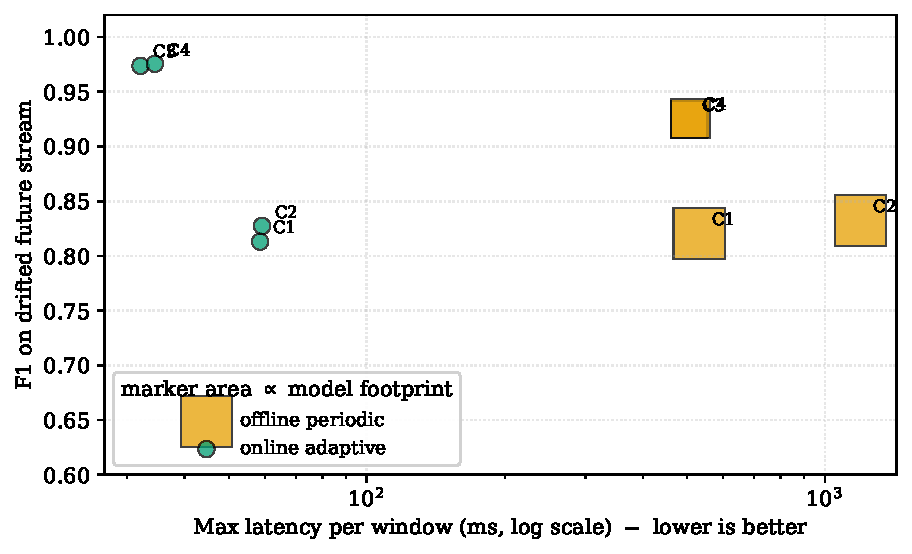
\includegraphics[width=0.86\textwidth]{fig_rq3_cost.pdf}
\caption{RQ4 cost/quality trade-off (periodic vs.\ online). The online learner (green) sits top-left---higher F1 at an order-of-magnitude lower tail latency---with a tiny footprint (marker area $\propto$ model size), while periodic retraining (orange) pays $\sim$600\,ms refit spikes and a multi-megabyte footprint for lower F1.}\label{fig:rq4cost}
\end{figure}

Table~\ref{tab:rq4-ratios} summarises the trade-off as ratios. The online model buys higher accuracy, far lower tail latency, a far smaller footprint and zero data-retention requirement, at the cost of modestly higher steady-state CPU. For any deployment with a per-window latency budget---which is to say any real-time detector behind an SLA---the bounded online profile is the safer engineering choice, independent of the accuracy advantage.

\begin{table}[t]
\caption{RQ4 cost ratios (periodic relative to online unless noted).}\label{tab:rq4-ratios}
\begin{tabular}{@{}lccccc@{}}
\toprule
Config & F1 gain (o$-$p) & Tail-lat.\ ratio & Size ratio & Retained (p vs.\ o) & CPU ratio (o/p) \\
\midrule
C1 & $+0.0600$ & 19.8$\times$ & 556.4$\times$ & 2880 vs.\ 0 & 5.7$\times$ \\
C2 & $+0.0571$ & 16.8$\times$ & 524.9$\times$ & 2880 vs.\ 0 & 5.8$\times$ \\
C3 & $+0.0913$ & 22.6$\times$ & 197.9$\times$ & 2880 vs.\ 0 & 5.7$\times$ \\
C4 & $+0.0929$ & 31.5$\times$ & 228.6$\times$ & 2880 vs.\ 0 & 4.4$\times$ \\
\bottomrule
\end{tabular}
\end{table}

\subsubsection{Adaptation behaviour}\label{sec:res-rq4-adapt}

Table~\ref{tab:rq4-adapt} reports how often the online model re-selects its champion configuration as drift appears. Richer telemetry requires \emph{fewer} corrective adapt events: with thin telemetry (C1) the model switches champions four times to keep up with drift, twice at C2, but once traces are added (C3/C4) the signal is rich enough that \emph{no} re-selection is needed at all. This is a second face of the completeness$\times$adaptation interaction: richer signal not only raises accuracy but stabilises the adaptation process, because more of the drift is explained by the EW normaliser and less must be chased by re-selecting the learner.

\begin{table}[t]
\caption{RQ4 online adaptation behaviour by configuration.}\label{tab:rq4-adapt}
\begin{tabular}{@{}lcccl@{}}
\toprule
Config & Features & Periodic refits & Online adapt events & Final champion \\
\midrule
C1 & 10 & 17 & 4 & $\eta_0{=}0.10,\ \alpha{=}10^{-4}$ \\
C2 & 14 & 17 & 2 & $\eta_0{=}0.01,\ \alpha{=}10^{-4}$ \\
C3 & 18 & 17 & 0 & $\eta_0{=}0.05,\ \alpha{=}10^{-4}$ \\
C4 & 23 & 17 & 0 & $\eta_0{=}0.05,\ \alpha{=}10^{-4}$ \\
\bottomrule
\end{tabular}
\end{table}

%%===========================================================%%
\section{Discussion}\label{sec:discussion}
%%===========================================================%%

\subsection{Drift, not completeness, is the deciding factor}\label{sec:disc-drift}

The juxtaposition of RQ1 and RQ4 is the paper's central message. On a stationary stream, completeness is decisive and the model is excellent regardless of paradigm: F1 climbs smoothly to $0.994$ (Table~\ref{tab:rq1}). On a drifted stream the same completeness barely moves the static model (Table~\ref{tab:rq4-head}); what determines whether the detector works is the learning policy. The static model's collapse is not a tuning failure that more telemetry or a better threshold could fix---it is structural. Once operations move the baseline, a boundary fitted to the old normal necessarily mislabels the new normal, and no amount of additional signal about the old normal helps. This reframes the field's guiding question. ``Does observability matter?'' has the answer ``yes, for the ceiling''; but ``what makes a detector work in production?'' has the answer ``keeping it current''. The two are complementary, and a study that varies only one axis can reach a misleading conclusion about the other.

\subsection{The completeness$\times$adaptation interaction}\label{sec:disc-interaction}

The two axes are not independent. Three results show their interaction. First, richness helps the online model far more than the static one ($+0.17$ vs.\ $+0.02$ from C1 to C4), so the benefit of instrumentation is itself \emph{contingent on adaptation}: a practitioner who invests in tracing but freezes the model captures almost none of the value (compare static C4 $=0.51$ with online C4 $=0.98$). Second, the online advantage over periodic widens with richness, because a continuous learner extracts more per window when each window carries more signal. Third, richer telemetry stabilises adaptation, reducing champion re-selections to zero once traces are present (Table~\ref{tab:rq4-adapt}). The practical reading is that observability investment and continual-learning investment should be made \emph{together}; either alone is sub-optimal, and the joint return exceeds the sum of the parts.

\subsection{Operational implications and an SLA framing}\label{sec:disc-ops}

Because RQ4 measures cost as well as accuracy, the choice of paradigm can be posed as a service-level decision. Periodic retraining, the field's usual concession to drift, is revealed as a partial, expensive and laggy patch: it lags by up to a retraining interval, must store a large labelled buffer (a data-governance liability as well as a memory cost), and stalls the pipeline with $\sim 600$ ms refit spikes that, behind a real-time SLA, are themselves an incident. The online model's per-window cost is bounded and small; its footprint is kilobytes; it retains no raw data, which simplifies privacy and retention compliance. Its only cost is higher aggregate CPU, spent smoothly. For a detector that must respond within a per-window budget, the bounded-latency profile is decisive on engineering grounds even before the accuracy advantage is considered. This connects directly to the practitioner guidance that observability is an exercise in managing cost as much as capability \cite{leadingobs,aws2022obs}.

The cost asymmetry, moreover, \emph{compounds} with scale rather than washing out. Consider the operational picture as the deployment grows from a handful of services to a large mesh. The periodic model's refit spike grows with the size of its training buffer and feature space, and its labelled-buffer footprint grows with both retention horizon and telemetry richness; every monitored service multiplies these costs, and each refit remains a synchronous stall that the surrounding pipeline must absorb. The online model's per-window update, by contrast, stays $O(d_c)$ and kilobyte-sized \emph{per detector} regardless of how long the stream has run, because it retains no history---the property that makes it cheap is structural, not a small-scale artefact. A fleet of online detectors therefore presents a flat, predictable resource profile that an operator can provision for, whereas a fleet of periodic detectors presents a sawtooth of refit spikes whose worst case is what capacity planning must target. In a production setting governed by tail latency and by the cost of over-provisioning for peaks, the bounded online profile is not merely preferable but materially cheaper to operate at scale, reinforcing the accuracy case rather than trading against it.

\subsection{When is periodic retraining acceptable?}\label{sec:disc-periodic}

The two cells in which periodic retraining edges the online model (scale-out under C1 and C2; Table~\ref{tab:rq4-regime}) are not a defect of the experiment but a boundary condition worth stating precisely, because it tells a practitioner when the cheaper, more familiar periodic approach suffices. Periodic retraining is competitive exactly when three conditions coincide: the drift is predominantly \emph{virtual} (the feature distribution moves but the concept does not), so that a refit on recent data restores the boundary without needing to relearn the decision; the telemetry is \emph{thin}, so that the online normaliser has few signals from which to re-centre continuously and its advantage is muted; and the operating environment can \emph{tolerate the tail-latency spikes and the labelled-buffer footprint} that periodic refitting imposes. The scale-out regime under metrics-only telemetry satisfies all three, and there periodic wins by a slim margin ($\sim 0.01$ F1). The moment any of the three fails---real concept drift (latency regression, $R_1$), richer telemetry (C3/C4), or a strict per-window latency budget---the online model regains a decisive and widening lead. The practical implication is not ``online always'', but ``online unless your drift is purely cosmetic, your telemetry is minimal, and your latency budget is loose''---a narrow and identifiable corner of the design space. For the common case of a richly-instrumented service subject to deployments (real drift) behind an SLA, online adaptation is the dominant choice on every axis we measured.

\subsection{Practical guidance}\label{sec:disc-guidance}

The results support concrete guidance.
\begin{itemize}
  \item \textbf{Minimum-viable observability for detection} is metrics${+}$logs${+}$traces (C3). Traces are the single highest-value increment for both detection (RQ1) and localisation (RQ3), and events/history add little to detection (C3$\approx$C4). A team constrained on instrumentation budget should prioritise tracing over event collection for the detection-and-localisation use case.
  \item \textbf{Continual learning is mandatory, not optional}, on any stream subject to deployments, autoscaling or load shifts---that is, essentially all production cloud-native systems. A frozen model is unsafe under drift irrespective of its telemetry (RQ4).
  \item \textbf{Prefer online to periodic} where a label signal is available and a per-window latency budget exists. Periodic retraining is acceptable only where labels arrive in large delayed batches and tail-latency spikes are tolerable.
  \item \textbf{Invest in observability and adaptation together.} The joint return exceeds either alone (\S\ref{sec:disc-interaction}).
\end{itemize}

These points compose into a short deployment checklist. \emph{(i)} Instrument to at least the three-pillar level (C3); budget for trace sampling rather than omitting traces, since traces are the decisive signal for both detection and localisation. \emph{(ii)} Choose the learning paradigm by interrogating the drift, not the model: if deployments and autoscaling routinely shift the baseline---real concept drift---a frozen model is disqualified regardless of its validation score. \emph{(iii)} Default to online adaptation with a bounded per-window update and a running normaliser; reserve periodic retraining for the narrow corner identified in \S\ref{sec:disc-periodic}. \emph{(iv)} Monitor the detector itself: track precision over time, because a precision decline with stable recall is the early signature of stale-normal drift (\S\ref{sec:res-rq4-prf}) and a trigger to verify that adaptation is keeping pace. \emph{(v)} Treat the labelled-data buffer of any periodic scheme as a governance liability, not just a memory cost, and prefer the zero-retention online design where data-handling constraints apply.

\subsection{Analysis by fault category}\label{sec:disc-faults}

The aggregate metrics conceal an instructive variation across the fault taxonomy that explains \emph{why} each pillar contributes what it does. Resource-exhaustion faults---memory leaks and CPU saturation---are largely metric-visible: they move CPU and memory utilisation directly, and even the metrics-only configuration detects them well, which is why C1 already attains F1 $\approx 0.91$ on the stationary set. Their localisation is the harder part, because resource pressure at one pod induces latency at its callers, smearing the metric signal across the dependency chain---precisely the ambiguity that the trace originating-error-span feature resolves (RQ3). Performance-degradation faults---latency spikes and error bursts---are where logs and traces earn their keep: an error burst raises the error-log count (a C2 feature) before it is unambiguous in the latency percentiles, and a latency spike that propagates is disentangled by span-level timing (a C3 feature). Availability faults---OOMKilled and CrashLoopBackOff---are the ones that motivate the events pillar: they manifest as discrete Kubernetes lifecycle events that no metric or log aggregate captures as cleanly, which is why C4 retains a localisation and robustness edge even though its detection F1 is statistically tied with C3 on the stationary set. The picture that emerges is that the pillars are not redundant but \emph{specialised}: each is the decisive signal for a different region of the fault taxonomy, and full MELT wins not by being uniformly better but by covering the union.

Under drift this specialisation interacts with the learning policy, and the per-regime breakdown (Table~\ref{tab:rq4-regime}) separates the two kinds of drift cleanly. The \emph{latency-regression} regime $R_1$ is real concept drift---a latency level that was anomalous becomes the new normal---and it is there that the static model collapses hardest (F1 $\approx 0.44$, its lowest at every configuration); richer telemetry does not rescue it, because the boundary, not merely the scaling, is now wrong. The \emph{scale-out} regime $R_2$ is predominantly virtual drift---the resource-utilisation baselines move but ``anomalous'' still means the same thing---and here the static model fares best of the three regimes (F1 up to $0.69$) and periodic refit even edges the online model under thin telemetry, because re-fitting on recent data restores the shifted scaling that a batch model needs. The \emph{combined-load} regime $R_3$ superimposes both. Only the online normaliser, which re-centres every feature continuously, neutralises the virtual component while incremental fitting tracks the conceptual one, which is why the online model holds F1 $\approx 0.79$--$0.99$ across $R_1$--$R_3$ where the static model never exceeds $0.69$ and bottoms at $0.44$.

\subsection{Relation to prior work}\label{sec:disc-prior}

Our stationary findings are consistent with, and sharpen, the literature. The monotonic completeness benefit echoes the general multimodal advantage reported by Han et al.\ \cite{han2024} and the multi-source gains of Chen et al.\ \cite{chen2025} and Wang et al.\ \cite{wang2018}, but---by holding the model fixed and varying only the signal set---attributes the largest single increment specifically to traces, which a fused-architecture comparison cannot do. The strength of ensemble trees on multimodal tabular telemetry (RQ2) corroborates the classical-ML results of Lomio et al.\ \cite{lomio2022} and extends them to the multimodal setting, while clarifying why a deep temporal model need not win when the windowed representation is already informative---consistent with the accuracy--cost concerns around VAE/temporal approaches such as Night's Watch \cite{dkmak2025}.

The drift findings (RQ4) speak to gaps the surveys identify but do not close. Raeiszadeh et al.\ \cite{raeiszadeh2026} name adaptability as a systematically unmet requirement; we quantify exactly what its absence costs (a collapse from $0.98$ to $0.51$) and what meeting it buys. Hrusto et al.\ \cite{hrusto2026} warn that single-snapshot, synthetic-distribution evaluation may not transfer; our two-axis design shows precisely \emph{how} it fails to transfer---the stationary ranking does not predict the drifted ranking---and offers a controlled-drift testbed as a middle path between synthetic-benchmark and uncontrolled-production evaluation. The industrial inadequacy of static thresholds reported by Islam et al.\ \cite{islam2021} is reproduced here as the stale-normal collapse and given a remedy. Finally, the proactive, observability-integrated framing of Mart et al.\ \cite{mart2020} is extended from \emph{forecasting} ahead of failure to \emph{continually re-learning} what failure looks like as the system changes.

\subsection{Threats to validity revisited}\label{sec:disc-threats}

The principal external-validity caveat is that the RQ4 stream, though drift-controlled and built on production-representative telemetry, is synthetic-prequential; absolute F1 values are testbed-specific. We stress that the contribution is the \emph{ordering and its reversal}, not the absolute numbers: that the stationary-best ranking does not survive drift, and that online dominates static at every cell and periodic in $10$ of $12$ regime$\times$configuration cells (the two exceptions being virtual-drift scale-out under thin telemetry), is robust to the absolute scale. The three-service topology limits topological generalisation and makes top-2 localisation uninformative (hence the top-1 focus). The online model depends on a usable label signal; where labels are scarce or heavily delayed, semi-supervised or unsupervised drift-adaptation would be required---a direction for future work. Finally, a single seed underlies the reported run; the effect sizes are large relative to plausible seed variance, but a multi-seed study would tighten the conclusion-validity argument.

It is worth being explicit about what a full real-deployment validation would add, and why we regard the present controlled study as the necessary first step rather than a substitute. On a live production stream, drift is neither scheduled nor labelled: regime changes arrive unannounced and entangled, ground truth is partial and delayed (often reconstructed after the fact from incident timelines), and the fault distribution is long-tailed in ways no injection taxonomy fully reproduces. A field study would therefore measure something our testbed cannot---robustness to \emph{unknown} drift and to \emph{imperfect} labels---but at the price of the very thing that makes our central claim interpretable: the ability to attribute the reversal between the stationary and drifted rankings to drift alone, with the model, features, faults and seed held fixed. The two evidence types are complementary, and in the order presented: the controlled result establishes \emph{that} the learning paradigm dominates completeness under drift and \emph{why}; a subsequent field deployment would establish \emph{how much} of that advantage survives the additional noise of production. We read the present findings as a strong prior for that field study, not as a replacement for it, consistent with the synthetic-versus-operational tension that motivated the design \cite{hrusto2026,islam2021}.

%%===========================================================%%
\section{Conclusion and Future Work}\label{sec:conclusion}
%%===========================================================%%

This paper asked whether, for a non-stationary observability stream, the learning paradigm matters more than telemetry richness, and how the two interact. By crossing four nested telemetry configurations with three learning policies on a single production-representative, fault-injected, drift-controlled testbed, we reached a two-part answer. Under stationary conditions, completeness is decisive: detection F1 rises monotonically from $0.906$ to $0.994$, traces are the single most valuable increment, ensemble trees are the strongest family, and traces lift root-cause top-1 localisation to a perfect $1.0$. But under drift this ceiling does not survive a frozen model: the static detector collapses to F1 $\approx 0.49$--$0.51$ regardless of telemetry, periodic retraining only partially and expensively recovers, and a lightweight online-adaptive detector dominates every configuration and the large majority of regimes---reaching $\approx 0.98$ under full MELT, beating an all-regimes oracle---while being $17$--$32\times$ better on tail latency, $\sim 200$--$550\times$ smaller, and free of any data-retention requirement.

The synthesis is that telemetry completeness and continual learning are complementary, not substitutable. Richer signals raise the attainable ceiling and stabilise adaptation; only adaptation realises that ceiling on a live, drifting system. The field's guiding question, ``does observability matter?'', is therefore incomplete: observability matters for what is \emph{achievable}, but keeping the model current is what makes the achievable \emph{actual} in production. Practitioners should invest in observability (at least to the metrics${+}$logs${+}$traces level) and in continual learning \emph{together}, and should prefer bounded-latency online adaptation to bursty periodic retraining wherever a label signal and a latency budget coexist.

Future work follows four directions. First, \emph{label efficiency}: extend the online comparison to semi- and self-supervised drift adaptation for settings where ground-truth labels are scarce or delayed, removing the present dependence on a prompt label signal. Second, \emph{topological generalisation}: scale the testbed beyond three services and to richer call graphs, restoring top-$k$ localisation as a meaningful axis and testing whether trace-driven localisation remains complete as the mesh grows. Third, \emph{drift diversity}: broaden the regime set beyond latency/scale/load to include schema changes, dependency re-wiring and seasonal patterns, and pair the empirical study with explicit drift-detection signals. Fourth, \emph{operational integration}: close the loop from online detection through trace-driven localisation to automated remediation, drawing on the LLM- and Bayesian-network RCA directions of Pedroso et al.\ \cite{pedroso2025} and the holistic fusion of Han et al.\ \cite{han2024}, so that a continually-current detector feeds a continually-current responder. A fifth direction concerns \emph{explicit drift signalling}: the present online model adapts implicitly through its normaliser and champion bandit, but pairing it with a dedicated drift detector would let the system distinguish virtual from real drift at runtime---precisely the distinction that \S\ref{sec:disc-periodic} shows determines whether refitting or re-normalising is the right response---and could trigger heavier adaptation only when a genuine concept change is detected, conserving the steady-state CPU that is the online model's sole cost disadvantage. Finally, the comparison should be extended to \emph{multi-seed and multi-trace-load} runs to convert the large but single-seed effect sizes reported here into formal significance intervals, and to confirm that the paradigm ordering is invariant to the specific synthetic stream.

Taken together, these directions share a single thesis, which is the contribution we most wish to carry forward: in a non-stationary world, a detector is never finished being trained. The observability community has invested heavily in \emph{seeing} more of the system; the evidence here is that comparable investment in \emph{relearning} what is seen is what converts that visibility into reliable detection.

%%===========================================================%%

\begin{acks}
The authors thank colleagues at the School of Built Environment, Engineering and Computing, Leeds Beckett University, for discussion and feedback. No specific grant funded this work, and the authors declare no competing interests. The research involves no human participants or personal data; all data are generated on a self-contained testbed with fault injection confined to an isolated environment, in line with Leeds Beckett University research-ethics guidance. The testbed configuration and the result datasets supporting the findings are available from the authors on reasonable request.
\end{acks}

\bibliographystyle{ACM-Reference-Format}
\bibliography{sn-bibliography}

\appendix
\section{Full feature listing}\label{app:features}

Table~\ref{tab:appfeatures} enumerates the engineered features by configuration. All features are window-local aggregates computed over the fixed-length detection window; configurations are nested, so the features of a configuration are the union of its own row and all rows above it. The dimensionalities ($10, 14, 18, 23$) correspond to the cumulative counts of Table~\ref{tab:configs}.

\begin{table}[h]
\caption{Engineered features by pillar. Counts are per-pillar additions; cumulative totals are 10 (C1), 14 (C2), 18 (C3), 23 (C4).}\label{tab:appfeatures}
\begin{tabular}{@{}llp{0.5\textwidth}@{}}
\toprule
Pillar (config) & \# & Features \\
\midrule
Metrics (C1) & 10 & CPU utilisation; memory utilisation; request rate; error rate; p50 latency; p95 latency; p99 latency; network bytes in; network bytes out; pod restart count \\
Logs (C2)    & 4  & total log volume; error-level log count; warning-level log count; log-template diversity (distinct templates per window) \\
Traces (C3)  & 4  & span rate; mean span duration; error-span rate; originating-error-span indicator (root of the error tree) \\
Events ${+}$ history (C4) & 5 & OOMKilled event count; CrashLoopBackOff event count; lifecycle restart-event count; rolling-baseline deviation (short horizon); rolling-baseline deviation (long horizon) \\
\bottomrule
\end{tabular}
\end{table}

\section{Experimental constants}\label{app:constants}

Table~\ref{tab:appconst} records the fixed parameters of the prequential RQ4 experiment, held constant across all telemetry configurations and learning policies.

\begin{table}[h]
\caption{Fixed experimental parameters.}\label{tab:appconst}
\begin{tabular}{@{}ll@{}}
\toprule
Parameter & Value \\
\midrule
Episodes                       & 320 \\
Windows evaluated              & 11{,}520 (2{,}880 warm-up $R_0$ ${+}$ 8{,}640 future) \\
Services                       & \texttt{movie-service}, \texttt{actor-service}, \texttt{review-service} \\
Regime sequence                & $R_0 \rightarrow R_1 \rightarrow R_2 \rightarrow R_3$ \\
Periodic retrain interval $\tau$ & every 500 windows (17 refits) \\
Periodic training buffer $B$   & 2{,}880 windows \\
Online candidate pool $\mathcal{H}$ & $\eta_0 \in \{0.01,0.05,0.1\}$, $\alpha \in \{10^{-4},10^{-3}\}$ \\
Evaluation protocol            & prequential (test-then-train) \\
Random seed                    & fixed (single deterministic run) \\
\bottomrule
\end{tabular}
\end{table}

\end{document}
